\documentclass{book}
\usepackage[a4paper,top=2.5cm,bottom=2.5cm,left=2.5cm,right=2.5cm]{geometry}
\usepackage{makeidx}
\usepackage{natbib}
\usepackage{graphicx}
\usepackage{multicol}
\usepackage{float}
\usepackage{listings}
\usepackage{color}
\usepackage{ifthen}
\usepackage[table]{xcolor}
\usepackage{textcomp}
\usepackage{alltt}
\usepackage{ifpdf}
\ifpdf
\usepackage[pdftex,
            pagebackref=true,
            colorlinks=true,
            linkcolor=blue,
            unicode
           ]{hyperref}
\else
\usepackage[ps2pdf,
            pagebackref=true,
            colorlinks=true,
            linkcolor=blue,
            unicode
           ]{hyperref}
\usepackage{pspicture}
\fi
\usepackage[utf8]{inputenc}
\usepackage{mathptmx}
\usepackage[scaled=.90]{helvet}
\usepackage{courier}
\usepackage{sectsty}
\usepackage[titles]{tocloft}
\usepackage{doxygen}
\lstset{language=C++,inputencoding=utf8,basicstyle=\footnotesize,breaklines=true,breakatwhitespace=true,tabsize=8,numbers=left }
\makeindex
\setcounter{tocdepth}{3}
\renewcommand{\footrulewidth}{0.4pt}
\renewcommand{\familydefault}{\sfdefault}
\hfuzz=15pt
\setlength{\emergencystretch}{15pt}
\hbadness=750
\tolerance=750
\begin{document}
\hypersetup{pageanchor=false,citecolor=blue}
\begin{titlepage}
\vspace*{7cm}
\begin{center}
{\Large Holy Balls }\\
\vspace*{1cm}
{\large Generated by Doxygen 1.8.0}\\
\vspace*{0.5cm}
{\small Sat Mar 31 2012 11:36:01}\\
\end{center}
\end{titlepage}
\clearemptydoublepage
\pagenumbering{roman}
\tableofcontents
\clearemptydoublepage
\pagenumbering{arabic}
\hypersetup{pageanchor=true,citecolor=blue}
\chapter{Class Index}
\section{Class Hierarchy}
This inheritance list is sorted roughly, but not completely, alphabetically\-:\begin{DoxyCompactList}
\item \contentsline{section}{Client}{\pageref{class_client}}{}
\item \contentsline{section}{collide\-\_\-event}{\pageref{structcollide__event}}{}
\item \contentsline{section}{funcobj$<$ R, I $>$}{\pageref{classfuncobj}}{}
\begin{DoxyCompactList}
\item \contentsline{section}{funcobjwrapper$<$ R, I, A $>$}{\pageref{classfuncobjwrapper}}{}
\end{DoxyCompactList}
\item \contentsline{section}{Game}{\pageref{class_game}}{}
\item \contentsline{section}{H\-B\-Map}{\pageref{class_h_b_map}}{}
\item \contentsline{section}{H\-B\-View\-Controller}{\pageref{class_h_b_view_controller}}{}
\begin{DoxyCompactList}
\item \contentsline{section}{Game\-View\-Controller}{\pageref{class_game_view_controller}}{}
\begin{DoxyCompactList}
\item \contentsline{section}{Holy\-Game\-View\-Controller}{\pageref{class_holy_game_view_controller}}{}
\item \contentsline{section}{Multi\-Game\-View\-Controller}{\pageref{class_multi_game_view_controller}}{}
\item \contentsline{section}{Unholy\-Game\-View\-Controller}{\pageref{class_unholy_game_view_controller}}{}
\end{DoxyCompactList}
\item \contentsline{section}{Server\-Connect\-View\-Controller}{\pageref{class_server_connect_view_controller}}{}
\item \contentsline{section}{Splash\-View\-Controller}{\pageref{class_splash_view_controller}}{}
\end{DoxyCompactList}
\item \contentsline{section}{leavefunc}{\pageref{classleavefunc}}{}
\item \contentsline{section}{Light}{\pageref{class_light}}{}
\item \contentsline{section}{Material}{\pageref{class_material}}{}
\begin{DoxyCompactList}
\item \contentsline{section}{Color}{\pageref{class_color}}{}
\item \contentsline{section}{Texture}{\pageref{class_texture}}{}
\end{DoxyCompactList}
\item \contentsline{section}{menu}{\pageref{classmenu}}{}
\item \contentsline{section}{menuitem}{\pageref{classmenuitem}}{}
\begin{DoxyCompactList}
\item \contentsline{section}{actionmenuitem}{\pageref{classactionmenuitem}}{}
\item \contentsline{section}{inputmenuitem}{\pageref{classinputmenuitem}}{}
\item \contentsline{section}{slidermenuitem}{\pageref{classslidermenuitem}}{}
\item \contentsline{section}{submenuitem}{\pageref{classsubmenuitem}}{}
\item \contentsline{section}{togglemenuitem}{\pageref{classtogglemenuitem}}{}
\end{DoxyCompactList}
\item \contentsline{section}{Object}{\pageref{class_object}}{}
\begin{DoxyCompactList}
\item \contentsline{section}{Rectangular\-Object}{\pageref{class_rectangular_object}}{}
\begin{DoxyCompactList}
\item \contentsline{section}{Rectangular\-Wall}{\pageref{class_rectangular_wall}}{}
\end{DoxyCompactList}
\item \contentsline{section}{Round\-Object}{\pageref{class_round_object}}{}
\end{DoxyCompactList}
\item \contentsline{section}{Obstacle}{\pageref{class_obstacle}}{}
\item \contentsline{section}{Parse\-Exception}{\pageref{class_parse_exception}}{}
\item \contentsline{section}{Player}{\pageref{class_player}}{}
\item \contentsline{section}{quitfunc}{\pageref{classquitfunc}}{}
\item \contentsline{section}{Read\-Packet}{\pageref{class_read_packet}}{}
\item \contentsline{section}{Socket}{\pageref{class_socket}}{}
\item \contentsline{section}{Socket\-Connection}{\pageref{class_socket_connection}}{}
\item \contentsline{section}{Spawn}{\pageref{class_spawn}}{}
\item \contentsline{section}{String\-Tokenizer}{\pageref{class_string_tokenizer}}{}
\item \contentsline{section}{Team}{\pageref{class_team}}{}
\item \contentsline{section}{textquad}{\pageref{structtextquad}}{}
\item \contentsline{section}{Vector2\-D}{\pageref{class_vector2_d}}{}
\item \contentsline{section}{Vector3\-D}{\pageref{class_vector3_d}}{}
\item \contentsline{section}{voidtype}{\pageref{structvoidtype}}{}
\item \contentsline{section}{World}{\pageref{class_world}}{}
\item \contentsline{section}{wrappedfuncobj$<$ R, I $>$}{\pageref{classwrappedfuncobj}}{}
\item \contentsline{section}{Write\-Packet}{\pageref{class_write_packet}}{}
\end{DoxyCompactList}

\chapter{Class Index}
\section{Class List}
Here are the classes, structs, unions and interfaces with brief descriptions\-:\begin{DoxyCompactList}
\item\contentsline{section}{\hyperlink{classactionmenuitem}{actionmenuitem} }{\pageref{classactionmenuitem}}{}
\item\contentsline{section}{\hyperlink{class_client}{Client} }{\pageref{class_client}}{}
\item\contentsline{section}{\hyperlink{structcollide__event}{collide\-\_\-event} }{\pageref{structcollide__event}}{}
\item\contentsline{section}{\hyperlink{class_color}{Color} }{\pageref{class_color}}{}
\item\contentsline{section}{\hyperlink{classfuncobj}{funcobj$<$ R, I $>$} }{\pageref{classfuncobj}}{}
\item\contentsline{section}{\hyperlink{classfuncobjwrapper}{funcobjwrapper$<$ R, I, A $>$} }{\pageref{classfuncobjwrapper}}{}
\item\contentsline{section}{\hyperlink{class_game}{Game} }{\pageref{class_game}}{}
\item\contentsline{section}{\hyperlink{class_game_view_controller}{Game\-View\-Controller} }{\pageref{class_game_view_controller}}{}
\item\contentsline{section}{\hyperlink{class_h_b_map}{H\-B\-Map} }{\pageref{class_h_b_map}}{}
\item\contentsline{section}{\hyperlink{class_h_b_view_controller}{H\-B\-View\-Controller} }{\pageref{class_h_b_view_controller}}{}
\item\contentsline{section}{\hyperlink{class_holy_game_view_controller}{Holy\-Game\-View\-Controller} }{\pageref{class_holy_game_view_controller}}{}
\item\contentsline{section}{\hyperlink{classinputmenuitem}{inputmenuitem} }{\pageref{classinputmenuitem}}{}
\item\contentsline{section}{\hyperlink{classleavefunc}{leavefunc} }{\pageref{classleavefunc}}{}
\item\contentsline{section}{\hyperlink{class_light}{Light} }{\pageref{class_light}}{}
\item\contentsline{section}{\hyperlink{class_material}{Material} }{\pageref{class_material}}{}
\item\contentsline{section}{\hyperlink{classmenu}{menu} }{\pageref{classmenu}}{}
\item\contentsline{section}{\hyperlink{classmenuitem}{menuitem} }{\pageref{classmenuitem}}{}
\item\contentsline{section}{\hyperlink{class_multi_game_view_controller}{Multi\-Game\-View\-Controller} }{\pageref{class_multi_game_view_controller}}{}
\item\contentsline{section}{\hyperlink{class_object}{Object} }{\pageref{class_object}}{}
\item\contentsline{section}{\hyperlink{class_obstacle}{Obstacle} }{\pageref{class_obstacle}}{}
\item\contentsline{section}{\hyperlink{class_parse_exception}{Parse\-Exception} }{\pageref{class_parse_exception}}{}
\item\contentsline{section}{\hyperlink{class_player}{Player} }{\pageref{class_player}}{}
\item\contentsline{section}{\hyperlink{classquitfunc}{quitfunc} }{\pageref{classquitfunc}}{}
\item\contentsline{section}{\hyperlink{class_read_packet}{Read\-Packet} }{\pageref{class_read_packet}}{}
\item\contentsline{section}{\hyperlink{class_rectangular_object}{Rectangular\-Object} }{\pageref{class_rectangular_object}}{}
\item\contentsline{section}{\hyperlink{class_rectangular_wall}{Rectangular\-Wall} }{\pageref{class_rectangular_wall}}{}
\item\contentsline{section}{\hyperlink{class_round_object}{Round\-Object} }{\pageref{class_round_object}}{}
\item\contentsline{section}{\hyperlink{class_server_connect_view_controller}{Server\-Connect\-View\-Controller} }{\pageref{class_server_connect_view_controller}}{}
\item\contentsline{section}{\hyperlink{classslidermenuitem}{slidermenuitem} }{\pageref{classslidermenuitem}}{}
\item\contentsline{section}{\hyperlink{class_socket}{Socket} }{\pageref{class_socket}}{}
\item\contentsline{section}{\hyperlink{class_socket_connection}{Socket\-Connection} }{\pageref{class_socket_connection}}{}
\item\contentsline{section}{\hyperlink{class_spawn}{Spawn} }{\pageref{class_spawn}}{}
\item\contentsline{section}{\hyperlink{class_splash_view_controller}{Splash\-View\-Controller} }{\pageref{class_splash_view_controller}}{}
\item\contentsline{section}{\hyperlink{class_string_tokenizer}{String\-Tokenizer} }{\pageref{class_string_tokenizer}}{}
\item\contentsline{section}{\hyperlink{classsubmenuitem}{submenuitem} }{\pageref{classsubmenuitem}}{}
\item\contentsline{section}{\hyperlink{class_team}{Team} }{\pageref{class_team}}{}
\item\contentsline{section}{\hyperlink{structtextquad}{textquad} }{\pageref{structtextquad}}{}
\item\contentsline{section}{\hyperlink{class_texture}{Texture} }{\pageref{class_texture}}{}
\item\contentsline{section}{\hyperlink{classtogglemenuitem}{togglemenuitem} }{\pageref{classtogglemenuitem}}{}
\item\contentsline{section}{\hyperlink{class_unholy_game_view_controller}{Unholy\-Game\-View\-Controller} }{\pageref{class_unholy_game_view_controller}}{}
\item\contentsline{section}{\hyperlink{class_vector2_d}{Vector2\-D} }{\pageref{class_vector2_d}}{}
\item\contentsline{section}{\hyperlink{class_vector3_d}{Vector3\-D} }{\pageref{class_vector3_d}}{}
\item\contentsline{section}{\hyperlink{structvoidtype}{voidtype} }{\pageref{structvoidtype}}{}
\item\contentsline{section}{\hyperlink{class_world}{World} }{\pageref{class_world}}{}
\item\contentsline{section}{\hyperlink{classwrappedfuncobj}{wrappedfuncobj$<$ R, I $>$} }{\pageref{classwrappedfuncobj}}{}
\item\contentsline{section}{\hyperlink{class_write_packet}{Write\-Packet} }{\pageref{class_write_packet}}{}
\end{DoxyCompactList}

\chapter{Class Documentation}
\hypertarget{classactionmenuitem}{\section{actionmenuitem Class Reference}
\label{classactionmenuitem}\index{actionmenuitem@{actionmenuitem}}
}
Inheritance diagram for actionmenuitem\-:\begin{figure}[H]
\begin{center}
\leavevmode
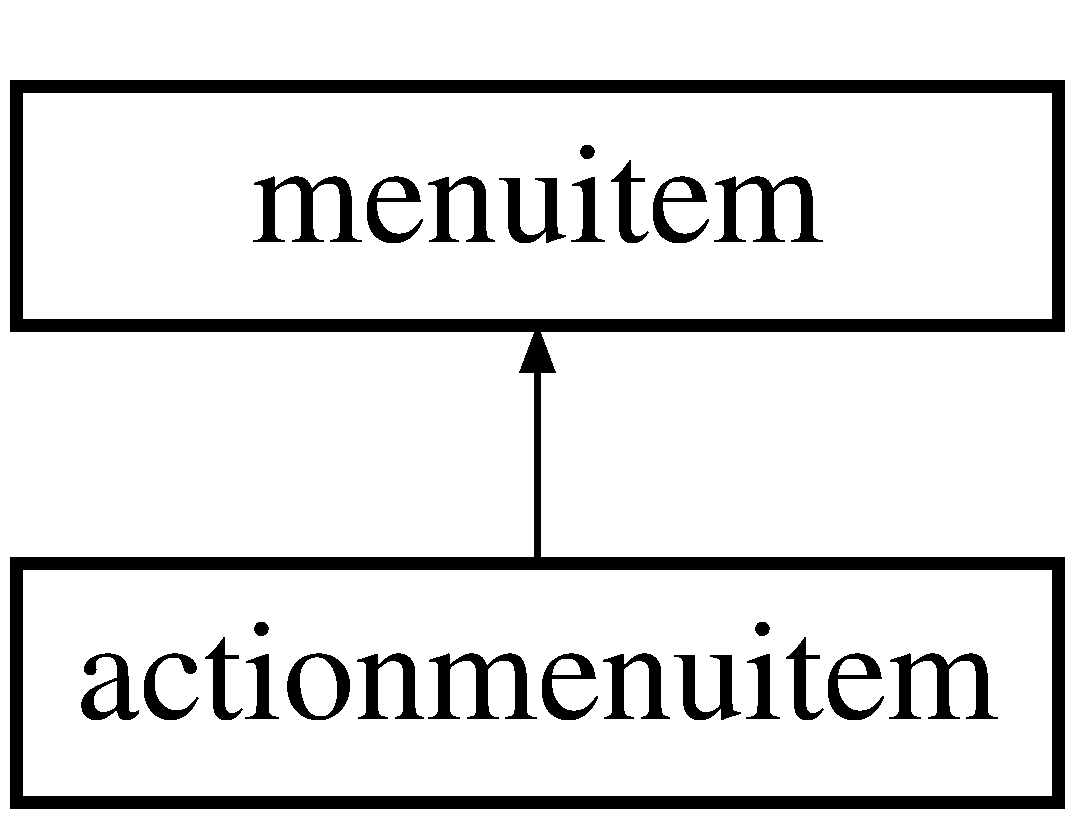
\includegraphics[height=2.000000cm]{classactionmenuitem}
\end{center}
\end{figure}
\subsection*{Public Member Functions}
\begin{DoxyCompactItemize}
\item 
\hypertarget{classactionmenuitem_a78dfdf114ebbfdebc7b983a2b3a7b4ea}{{\footnotesize template$<$class A $>$ }\\{\bfseries actionmenuitem} (A init1, char $\ast$name1)}\label{classactionmenuitem_a78dfdf114ebbfdebc7b983a2b3a7b4ea}

\item 
\hypertarget{classactionmenuitem_a91025817e7fdf766b4f2fae25759bba5}{virtual bool {\bfseries activate} ()}\label{classactionmenuitem_a91025817e7fdf766b4f2fae25759bba5}

\item 
\hypertarget{classactionmenuitem_accaa80b69c19704b420ff35bc044815f}{virtual bool {\bfseries should\-Menu\-Be\-Drawn} ()}\label{classactionmenuitem_accaa80b69c19704b420ff35bc044815f}

\end{DoxyCompactItemize}


The documentation for this class was generated from the following files\-:\begin{DoxyCompactItemize}
\item 
menu.\-h\item 
menuitem.\-cpp\end{DoxyCompactItemize}

\hypertarget{class_client}{\section{Client Class Reference}
\label{class_client}\index{Client@{Client}}
}
\subsection*{Public Attributes}
\begin{DoxyCompactItemize}
\item 
\hypertarget{class_client_a6eedc226499b6504156da363c454cc78}{\hyperlink{class_socket_connection}{Socket\-Connection} $\ast$ {\bfseries sc}}\label{class_client_a6eedc226499b6504156da363c454cc78}

\item 
\hypertarget{class_client_a81ec429197b559ebdc8d41c5c44557a4}{int {\bfseries latest\-Packet}}\label{class_client_a81ec429197b559ebdc8d41c5c44557a4}

\item 
\hypertarget{class_client_ab79ad95264939f089a2f0b8e0ca62d37}{int {\bfseries id}}\label{class_client_ab79ad95264939f089a2f0b8e0ca62d37}

\end{DoxyCompactItemize}


The documentation for this class was generated from the following file\-:\begin{DoxyCompactItemize}
\item 
server.\-h\end{DoxyCompactItemize}

\hypertarget{structcollide__event}{\section{collide\-\_\-event Struct Reference}
\label{structcollide__event}\index{collide\-\_\-event@{collide\-\_\-event}}
}
\subsection*{Public Attributes}
\begin{DoxyCompactItemize}
\item 
\hypertarget{structcollide__event_acf94b262e702e090fb9b7deea3f81267}{float {\bfseries time}}\label{structcollide__event_acf94b262e702e090fb9b7deea3f81267}

\item 
\hypertarget{structcollide__event_a62c3ceb5b04061647ecdd123b0c5be8b}{int {\bfseries type}}\label{structcollide__event_a62c3ceb5b04061647ecdd123b0c5be8b}

\item 
\hypertarget{structcollide__event_a54c3a2edee7604746815f795c9eed61e}{int {\bfseries t1}}\label{structcollide__event_a54c3a2edee7604746815f795c9eed61e}

\item 
\hypertarget{structcollide__event_ab871578e8f2ec7953bfbb32ecf27e650}{int {\bfseries t2}}\label{structcollide__event_ab871578e8f2ec7953bfbb32ecf27e650}

\end{DoxyCompactItemize}


The documentation for this struct was generated from the following file\-:\begin{DoxyCompactItemize}
\item 
simulate.\-cpp\end{DoxyCompactItemize}

\hypertarget{class_color}{\section{Color Class Reference}
\label{class_color}\index{Color@{Color}}
}
\subsection*{Public Member Functions}
\begin{DoxyCompactItemize}
\item 
\hypertarget{class_color_a8e195b730ea2cd93d19012b9297ca368}{{\bfseries Color} (unsigned char x=0, unsigned char y=0, unsigned char z=0)}\label{class_color_a8e195b730ea2cd93d19012b9297ca368}

\end{DoxyCompactItemize}
\subsection*{Public Attributes}
\begin{DoxyCompactItemize}
\item 
\hypertarget{class_color_ab9a9c7134511f9b116a6fcc81a303ba6}{unsigned char {\bfseries r}}\label{class_color_ab9a9c7134511f9b116a6fcc81a303ba6}

\item 
\hypertarget{class_color_adc506c5063609cacdda2c007da3b7a5f}{unsigned char {\bfseries g}}\label{class_color_adc506c5063609cacdda2c007da3b7a5f}

\item 
\hypertarget{class_color_a9f00605f7024dcb79342e97fae52c1bd}{unsigned char {\bfseries b}}\label{class_color_a9f00605f7024dcb79342e97fae52c1bd}

\item 
\hypertarget{class_color_a39bb1f3f9a514ac1a581ca27fddebebc}{unsigned char {\bfseries a}}\label{class_color_a39bb1f3f9a514ac1a581ca27fddebebc}

\end{DoxyCompactItemize}


The documentation for this class was generated from the following file\-:\begin{DoxyCompactItemize}
\item 
hack.\-h\end{DoxyCompactItemize}

\hypertarget{classfuncobj}{\section{funcobj$<$ R, I $>$ Class Template Reference}
\label{classfuncobj}\index{funcobj$<$ R, I $>$@{funcobj$<$ R, I $>$}}
}
Inheritance diagram for funcobj$<$ R, I $>$\-:\begin{figure}[H]
\begin{center}
\leavevmode
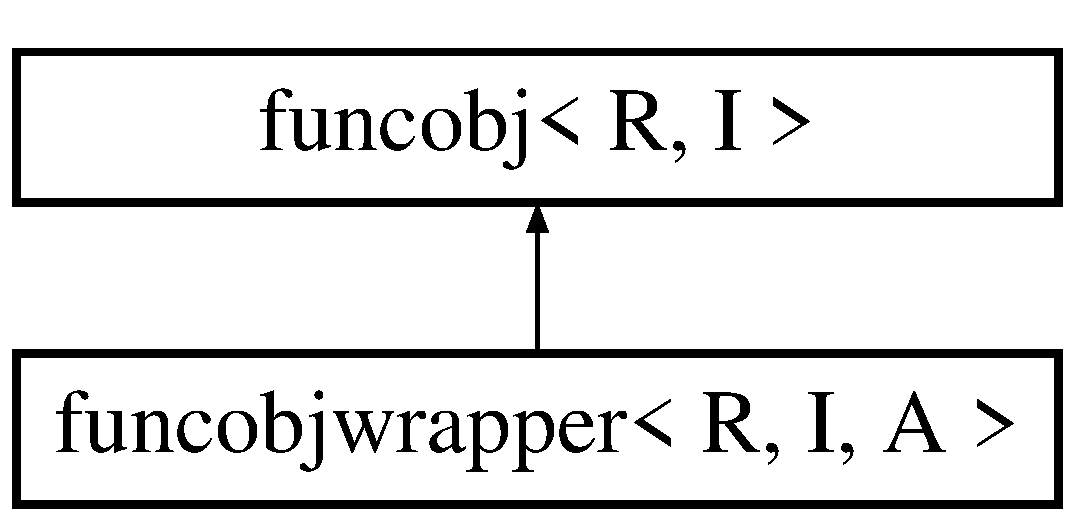
\includegraphics[height=2.000000cm]{classfuncobj}
\end{center}
\end{figure}
\subsection*{Public Member Functions}
\begin{DoxyCompactItemize}
\item 
\hypertarget{classfuncobj_ad8311f20bd0ddd211fec6e97847eccf3}{virtual R {\bfseries operator()} (I)=0}\label{classfuncobj_ad8311f20bd0ddd211fec6e97847eccf3}

\end{DoxyCompactItemize}
\subsubsection*{template$<$class R, class I$>$ class funcobj$<$ R, I $>$}



The documentation for this class was generated from the following file\-:\begin{DoxyCompactItemize}
\item 
menu.\-h\end{DoxyCompactItemize}

\hypertarget{classfuncobjwrapper}{\section{funcobjwrapper$<$ R, I, A $>$ Class Template Reference}
\label{classfuncobjwrapper}\index{funcobjwrapper$<$ R, I, A $>$@{funcobjwrapper$<$ R, I, A $>$}}
}
Inheritance diagram for funcobjwrapper$<$ R, I, A $>$\-:\begin{figure}[H]
\begin{center}
\leavevmode
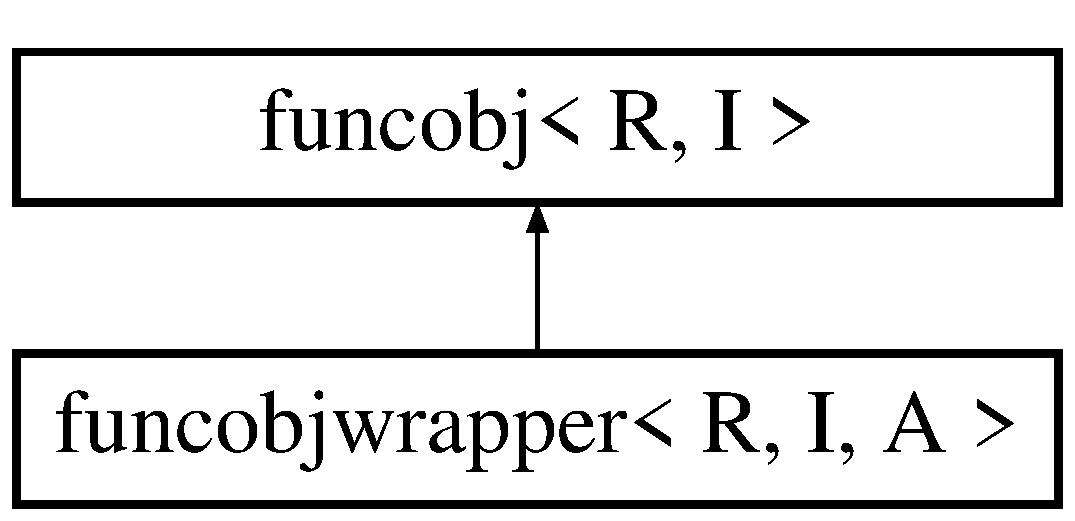
\includegraphics[height=2.000000cm]{classfuncobjwrapper}
\end{center}
\end{figure}
\subsection*{Public Member Functions}
\begin{DoxyCompactItemize}
\item 
\hypertarget{classfuncobjwrapper_a3824a1feca3b6905bc87881f85946c69}{{\bfseries funcobjwrapper} (A internal)}\label{classfuncobjwrapper_a3824a1feca3b6905bc87881f85946c69}

\item 
\hypertarget{classfuncobjwrapper_a5b6f835278f661b86c3fc6eb54e0d506}{R {\bfseries operator()} (I i)}\label{classfuncobjwrapper_a5b6f835278f661b86c3fc6eb54e0d506}

\end{DoxyCompactItemize}
\subsubsection*{template$<$class R, class I, class A$>$ class funcobjwrapper$<$ R, I, A $>$}



The documentation for this class was generated from the following file\-:\begin{DoxyCompactItemize}
\item 
menu.\-h\end{DoxyCompactItemize}

\hypertarget{class_game}{\section{Game Class Reference}
\label{class_game}\index{Game@{Game}}
}
\subsection*{Public Member Functions}
\begin{DoxyCompactItemize}
\item 
\hypertarget{class_game_a5a53fbc1ec712cd70ecc54f1d07c390b}{bool {\bfseries add\-\_\-player} (\hyperlink{class_client}{Client} cl)}\label{class_game_a5a53fbc1ec712cd70ecc54f1d07c390b}

\item 
\hypertarget{class_game_aebddf723758c118c2693f58d9dca3b52}{void {\bfseries remove\-\_\-player} (int id)}\label{class_game_aebddf723758c118c2693f58d9dca3b52}

\item 
\hypertarget{class_game_a5758f33d3f7da202aef70865025714c2}{void {\bfseries send\-\_\-world} ()}\label{class_game_a5758f33d3f7da202aef70865025714c2}

\item 
\hypertarget{class_game_a9ec2affa9074115ddf6053d7338cfbb5}{void {\bfseries send\-\_\-sounds\-\_\-to} (\hyperlink{class_socket_connection}{Socket\-Connection} $\ast$c)}\label{class_game_a9ec2affa9074115ddf6053d7338cfbb5}

\item 
\hypertarget{class_game_a1b351b4b7f892c69709a99c96ab6a88d}{void {\bfseries process\-\_\-packet} (int id, \hyperlink{class_read_packet}{Read\-Packet} $\ast$rp)}\label{class_game_a1b351b4b7f892c69709a99c96ab6a88d}

\item 
\hypertarget{class_game_a2648dc91da0dd1424d5b7c45510515a0}{void {\bfseries update} (float dt)}\label{class_game_a2648dc91da0dd1424d5b7c45510515a0}

\end{DoxyCompactItemize}


The documentation for this class was generated from the following files\-:\begin{DoxyCompactItemize}
\item 
game.\-h\item 
game.\-cpp\end{DoxyCompactItemize}

\hypertarget{class_game_view_controller}{\section{Game\-View\-Controller Class Reference}
\label{class_game_view_controller}\index{Game\-View\-Controller@{Game\-View\-Controller}}
}
Inheritance diagram for Game\-View\-Controller\-:\begin{figure}[H]
\begin{center}
\leavevmode
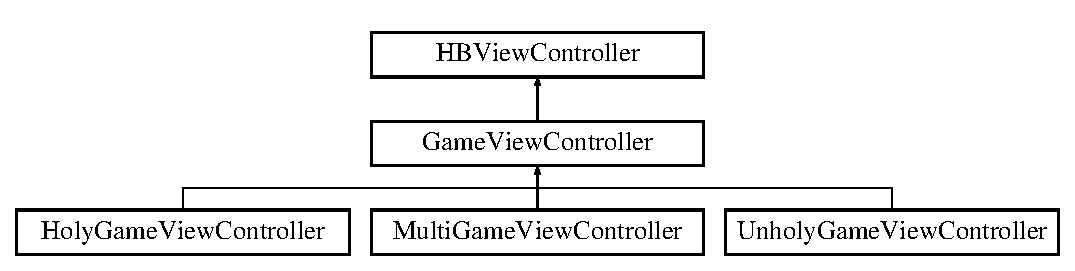
\includegraphics[height=3.000000cm]{class_game_view_controller}
\end{center}
\end{figure}
\subsection*{Public Member Functions}
\begin{DoxyCompactItemize}
\item 
\hypertarget{class_game_view_controller_a9cc7d13073c12187e8c7d9aa89727f31}{H\-B\-View\-Mode {\bfseries did\-Finish\-View} ()}\label{class_game_view_controller_a9cc7d13073c12187e8c7d9aa89727f31}

\item 
\hypertarget{class_game_view_controller_a6cb003b6eaf79a580a60d9957274023c}{void {\bfseries process} ()}\label{class_game_view_controller_a6cb003b6eaf79a580a60d9957274023c}

\item 
\hypertarget{class_game_view_controller_a92ffa5042982ee85cf302aea16f5e3ca}{void {\bfseries render} ()}\label{class_game_view_controller_a92ffa5042982ee85cf302aea16f5e3ca}

\item 
\hypertarget{class_game_view_controller_a628bd4d9a18bc85f6ce675cf138dbdf0}{bool {\bfseries quit} ()}\label{class_game_view_controller_a628bd4d9a18bc85f6ce675cf138dbdf0}

\item 
\hypertarget{class_game_view_controller_a93c9963feef7c3558632b2cec9264045}{bool {\bfseries leave} ()}\label{class_game_view_controller_a93c9963feef7c3558632b2cec9264045}

\end{DoxyCompactItemize}
\subsection*{Protected Attributes}
\begin{DoxyCompactItemize}
\item 
\hypertarget{class_game_view_controller_a91c0ce553ca7a678d5233dcfabee8bde}{unsigned int {\bfseries albuf} \mbox{[}3\mbox{]}}\label{class_game_view_controller_a91c0ce553ca7a678d5233dcfabee8bde}

\item 
\hypertarget{class_game_view_controller_a1d9116b19165481a2d7b2fd293c70ba8}{unsigned int {\bfseries alsrcs} \mbox{[}A\-L\-S\-R\-C\-S\mbox{]}}\label{class_game_view_controller_a1d9116b19165481a2d7b2fd293c70ba8}

\item 
\hypertarget{class_game_view_controller_afb4caa9132e818258847f9e26af91caa}{\hyperlink{class_socket}{Socket} $\ast$ {\bfseries sock}}\label{class_game_view_controller_afb4caa9132e818258847f9e26af91caa}

\item 
\hypertarget{class_game_view_controller_a119f27e5e8a55c3115014f361990dee3}{\hyperlink{class_socket_connection}{Socket\-Connection} $\ast$ {\bfseries sc}}\label{class_game_view_controller_a119f27e5e8a55c3115014f361990dee3}

\item 
\hypertarget{class_game_view_controller_a4efe8765e88b7add40916adbb6ae7605}{\hyperlink{class_world}{World} {\bfseries world}}\label{class_game_view_controller_a4efe8765e88b7add40916adbb6ae7605}

\item 
\hypertarget{class_game_view_controller_ad326ed913266f1fd3c55bf8abcce21e2}{float {\bfseries angle}}\label{class_game_view_controller_ad326ed913266f1fd3c55bf8abcce21e2}

\item 
\hypertarget{class_game_view_controller_a2400b43abdd6abed1275c198b1ba43da}{int {\bfseries my\-Id}}\label{class_game_view_controller_a2400b43abdd6abed1275c198b1ba43da}

\item 
\hypertarget{class_game_view_controller_a78d274d7647995fee5b3573229e0c622}{int {\bfseries latest\-Packet}}\label{class_game_view_controller_a78d274d7647995fee5b3573229e0c622}

\item 
\hypertarget{class_game_view_controller_a7cbc2ea5527a2f0f4b0c0c6ec1555a93}{int {\bfseries count}}\label{class_game_view_controller_a7cbc2ea5527a2f0f4b0c0c6ec1555a93}

\item 
\hypertarget{class_game_view_controller_a39a60f61eea22078c9b5371971b7a0c0}{int {\bfseries old\-Time}}\label{class_game_view_controller_a39a60f61eea22078c9b5371971b7a0c0}

\item 
\hypertarget{class_game_view_controller_aab32bff4f1a3b3c12279ce6c29eaef86}{\hyperlink{classmenu}{menu} $\ast$ {\bfseries mainmenu}}\label{class_game_view_controller_aab32bff4f1a3b3c12279ce6c29eaef86}

\item 
\hypertarget{class_game_view_controller_a3441dd8397265ff7c9fc81a6445603b2}{A\-Lfloat {\bfseries pos} \mbox{[}3\mbox{]}}\label{class_game_view_controller_a3441dd8397265ff7c9fc81a6445603b2}

\item 
\hypertarget{class_game_view_controller_a722c13809b23d45f591651ae4581d593}{A\-Lfloat {\bfseries vel} \mbox{[}3\mbox{]}}\label{class_game_view_controller_a722c13809b23d45f591651ae4581d593}

\item 
\hypertarget{class_game_view_controller_ad8a34e8ebc038a6dac34fb77eb0ace30}{A\-Lfloat {\bfseries ori} \mbox{[}6\mbox{]}}\label{class_game_view_controller_ad8a34e8ebc038a6dac34fb77eb0ace30}

\end{DoxyCompactItemize}


The documentation for this class was generated from the following files\-:\begin{DoxyCompactItemize}
\item 
Game\-View\-Controller.\-h\item 
Game\-View\-Controller.\-cpp\end{DoxyCompactItemize}

\hypertarget{class_h_b_map}{\section{H\-B\-Map Class Reference}
\label{class_h_b_map}\index{H\-B\-Map@{H\-B\-Map}}
}
\subsection*{Public Member Functions}
\begin{DoxyCompactItemize}
\item 
\hyperlink{class_h_b_map_ac67b05db88443e2d7044f134864d2f53}{H\-B\-Map} ()
\item 
\hyperlink{class_h_b_map_a368322ab6cbd98123a00e5df1822d204}{H\-B\-Map} (std\-::string filename)
\item 
unsigned \hyperlink{class_h_b_map_a515e8a0be2e7cce366a81632cce6da4d}{get\-Width} ()
\item 
unsigned \hyperlink{class_h_b_map_a5935af936a849f70c66b0830d517a4c9}{get\-Height} ()
\item 
std\-::string \& \hyperlink{class_h_b_map_a306c703d78a5be354f73186eb9f0cf4c}{get\-Name} ()
\item 
std\-::vector$<$ Game\-Mode $>$ \& \hyperlink{class_h_b_map_a86c9120ba5dea97040c019e99daa0226}{get\-Game\-Modes} ()
\item 
std\-::vector$<$ \hyperlink{struct_team}{Team} $>$ \& \hyperlink{class_h_b_map_a17d50199fdc09f1c8fac6b49d2989cbf}{get\-Teams} ()
\item 
std\-::vector$<$ \hyperlink{class_obstacle}{Obstacle} $>$ \& \hyperlink{class_h_b_map_abf3a3b5a59ba22a08d51ef94cc44794d}{get\-Spawns\-For\-Team} (unsigned team)
\item 
std\-::vector$<$ \hyperlink{class_spawn}{Spawn} $>$ \& \hyperlink{class_h_b_map_a841fd545b388d50df1755f788dee9a03}{get\-Flags\-For\-Team} (unsigned team)
\item 
std\-::vector$<$ \hyperlink{class_obstacle}{Obstacle} $>$ \& \hyperlink{class_h_b_map_adb7096539acd9c192b8291bcea719191}{get\-Walls} ()
\end{DoxyCompactItemize}
\subsection*{Static Public Attributes}
\begin{DoxyCompactItemize}
\item 
static const unsigned \hyperlink{class_h_b_map_a86583aaa4db0d7bac49b94d48cdefc86}{M\-A\-X\-\_\-\-T\-E\-A\-M\-S} = 10
\end{DoxyCompactItemize}


\subsection{Constructor \& Destructor Documentation}
\hypertarget{class_h_b_map_ac67b05db88443e2d7044f134864d2f53}{\index{H\-B\-Map@{H\-B\-Map}!H\-B\-Map@{H\-B\-Map}}
\index{H\-B\-Map@{H\-B\-Map}!HBMap@{H\-B\-Map}}
\subsubsection[{H\-B\-Map}]{\setlength{\rightskip}{0pt plus 5cm}{\bf H\-B\-Map\-::\-H\-B\-Map} (
\begin{DoxyParamCaption}
{}
\end{DoxyParamCaption}
)\hspace{0.3cm}{\ttfamily  \mbox{[}inline\mbox{]}}}}\label{class_h_b_map_ac67b05db88443e2d7044f134864d2f53}
Empty constructor that does nothing. \hypertarget{class_h_b_map_a368322ab6cbd98123a00e5df1822d204}{\index{H\-B\-Map@{H\-B\-Map}!H\-B\-Map@{H\-B\-Map}}
\index{H\-B\-Map@{H\-B\-Map}!HBMap@{H\-B\-Map}}
\subsubsection[{H\-B\-Map}]{\setlength{\rightskip}{0pt plus 5cm}{\bf H\-B\-Map\-::\-H\-B\-Map} (
\begin{DoxyParamCaption}
\item[{std\-::string}]{filename}
\end{DoxyParamCaption}
)\hspace{0.3cm}{\ttfamily  \mbox{[}inline\mbox{]}}}}\label{class_h_b_map_a368322ab6cbd98123a00e5df1822d204}
Creates an \hyperlink{class_h_b_map}{H\-B\-Map} instance given the map filename.


\begin{DoxyExceptions}{Exceptions}
{\em \hyperlink{class_parse_exception}{Parse\-Exception}} & when the parser encounters invalid syntax. \\
\hline
\end{DoxyExceptions}


\subsection{Member Function Documentation}
\hypertarget{class_h_b_map_a841fd545b388d50df1755f788dee9a03}{\index{H\-B\-Map@{H\-B\-Map}!get\-Flags\-For\-Team@{get\-Flags\-For\-Team}}
\index{get\-Flags\-For\-Team@{get\-Flags\-For\-Team}!HBMap@{H\-B\-Map}}
\subsubsection[{get\-Flags\-For\-Team}]{\setlength{\rightskip}{0pt plus 5cm}std\-::vector$<${\bf Spawn}$>$\& {\bf H\-B\-Map\-::get\-Flags\-For\-Team} (
\begin{DoxyParamCaption}
\item[{unsigned}]{team}
\end{DoxyParamCaption}
)\hspace{0.3cm}{\ttfamily  \mbox{[}inline\mbox{]}}}}\label{class_h_b_map_a841fd545b388d50df1755f788dee9a03}
Gets the flags for a given team.


\begin{DoxyParams}{Parameters}
{\em team} & the team number for which to get flags.\\
\hline
\end{DoxyParams}
\begin{DoxyReturn}{Returns}
the flags for team. 
\end{DoxyReturn}
\hypertarget{class_h_b_map_a86c9120ba5dea97040c019e99daa0226}{\index{H\-B\-Map@{H\-B\-Map}!get\-Game\-Modes@{get\-Game\-Modes}}
\index{get\-Game\-Modes@{get\-Game\-Modes}!HBMap@{H\-B\-Map}}
\subsubsection[{get\-Game\-Modes}]{\setlength{\rightskip}{0pt plus 5cm}std\-::vector$<$Game\-Mode$>$\& {\bf H\-B\-Map\-::get\-Game\-Modes} (
\begin{DoxyParamCaption}
{}
\end{DoxyParamCaption}
)\hspace{0.3cm}{\ttfamily  \mbox{[}inline\mbox{]}}}}\label{class_h_b_map_a86c9120ba5dea97040c019e99daa0226}
Gets the game modes of the map.

\begin{DoxyReturn}{Returns}
the game modes in no particular order. 
\end{DoxyReturn}
\hypertarget{class_h_b_map_a5935af936a849f70c66b0830d517a4c9}{\index{H\-B\-Map@{H\-B\-Map}!get\-Height@{get\-Height}}
\index{get\-Height@{get\-Height}!HBMap@{H\-B\-Map}}
\subsubsection[{get\-Height}]{\setlength{\rightskip}{0pt plus 5cm}unsigned {\bf H\-B\-Map\-::get\-Height} (
\begin{DoxyParamCaption}
{}
\end{DoxyParamCaption}
)\hspace{0.3cm}{\ttfamily  \mbox{[}inline\mbox{]}}}}\label{class_h_b_map_a5935af936a849f70c66b0830d517a4c9}
Gets the height of the map.

\begin{DoxyReturn}{Returns}
the height. 
\end{DoxyReturn}
\hypertarget{class_h_b_map_a306c703d78a5be354f73186eb9f0cf4c}{\index{H\-B\-Map@{H\-B\-Map}!get\-Name@{get\-Name}}
\index{get\-Name@{get\-Name}!HBMap@{H\-B\-Map}}
\subsubsection[{get\-Name}]{\setlength{\rightskip}{0pt plus 5cm}std\-::string\& {\bf H\-B\-Map\-::get\-Name} (
\begin{DoxyParamCaption}
{}
\end{DoxyParamCaption}
)\hspace{0.3cm}{\ttfamily  \mbox{[}inline\mbox{]}}}}\label{class_h_b_map_a306c703d78a5be354f73186eb9f0cf4c}
Gets the name of the map.

\begin{DoxyReturn}{Returns}
the name. 
\end{DoxyReturn}
\hypertarget{class_h_b_map_abf3a3b5a59ba22a08d51ef94cc44794d}{\index{H\-B\-Map@{H\-B\-Map}!get\-Spawns\-For\-Team@{get\-Spawns\-For\-Team}}
\index{get\-Spawns\-For\-Team@{get\-Spawns\-For\-Team}!HBMap@{H\-B\-Map}}
\subsubsection[{get\-Spawns\-For\-Team}]{\setlength{\rightskip}{0pt plus 5cm}std\-::vector$<${\bf Obstacle}$>$\& {\bf H\-B\-Map\-::get\-Spawns\-For\-Team} (
\begin{DoxyParamCaption}
\item[{unsigned}]{team}
\end{DoxyParamCaption}
)\hspace{0.3cm}{\ttfamily  \mbox{[}inline\mbox{]}}}}\label{class_h_b_map_abf3a3b5a59ba22a08d51ef94cc44794d}
Gets the spawns for a given team.


\begin{DoxyParams}{Parameters}
{\em team} & the team number for which to get spawns.\\
\hline
\end{DoxyParams}
\begin{DoxyReturn}{Returns}
the spawns for team. 
\end{DoxyReturn}
\hypertarget{class_h_b_map_a17d50199fdc09f1c8fac6b49d2989cbf}{\index{H\-B\-Map@{H\-B\-Map}!get\-Teams@{get\-Teams}}
\index{get\-Teams@{get\-Teams}!HBMap@{H\-B\-Map}}
\subsubsection[{get\-Teams}]{\setlength{\rightskip}{0pt plus 5cm}std\-::vector$<${\bf Team}$>$\& {\bf H\-B\-Map\-::get\-Teams} (
\begin{DoxyParamCaption}
{}
\end{DoxyParamCaption}
)\hspace{0.3cm}{\ttfamily  \mbox{[}inline\mbox{]}}}}\label{class_h_b_map_a17d50199fdc09f1c8fac6b49d2989cbf}
Gets the team list and properties of the map.

\begin{DoxyReturn}{Returns}
the team list containing \hyperlink{struct_team}{Team} objects in no particular order. 
\end{DoxyReturn}
\hypertarget{class_h_b_map_adb7096539acd9c192b8291bcea719191}{\index{H\-B\-Map@{H\-B\-Map}!get\-Walls@{get\-Walls}}
\index{get\-Walls@{get\-Walls}!HBMap@{H\-B\-Map}}
\subsubsection[{get\-Walls}]{\setlength{\rightskip}{0pt plus 5cm}std\-::vector$<${\bf Obstacle}$>$\& {\bf H\-B\-Map\-::get\-Walls} (
\begin{DoxyParamCaption}
{}
\end{DoxyParamCaption}
)\hspace{0.3cm}{\ttfamily  \mbox{[}inline\mbox{]}}}}\label{class_h_b_map_adb7096539acd9c192b8291bcea719191}
Gets the walls for the map.

\begin{DoxyReturn}{Returns}
a list of walls. 
\end{DoxyReturn}
\hypertarget{class_h_b_map_a515e8a0be2e7cce366a81632cce6da4d}{\index{H\-B\-Map@{H\-B\-Map}!get\-Width@{get\-Width}}
\index{get\-Width@{get\-Width}!HBMap@{H\-B\-Map}}
\subsubsection[{get\-Width}]{\setlength{\rightskip}{0pt plus 5cm}unsigned {\bf H\-B\-Map\-::get\-Width} (
\begin{DoxyParamCaption}
{}
\end{DoxyParamCaption}
)\hspace{0.3cm}{\ttfamily  \mbox{[}inline\mbox{]}}}}\label{class_h_b_map_a515e8a0be2e7cce366a81632cce6da4d}
Gets the width of the map.

\begin{DoxyReturn}{Returns}
the width. 
\end{DoxyReturn}


\subsection{Member Data Documentation}
\hypertarget{class_h_b_map_a86583aaa4db0d7bac49b94d48cdefc86}{\index{H\-B\-Map@{H\-B\-Map}!M\-A\-X\-\_\-\-T\-E\-A\-M\-S@{M\-A\-X\-\_\-\-T\-E\-A\-M\-S}}
\index{M\-A\-X\-\_\-\-T\-E\-A\-M\-S@{M\-A\-X\-\_\-\-T\-E\-A\-M\-S}!HBMap@{H\-B\-Map}}
\subsubsection[{M\-A\-X\-\_\-\-T\-E\-A\-M\-S}]{\setlength{\rightskip}{0pt plus 5cm}const unsigned {\bf H\-B\-Map\-::\-M\-A\-X\-\_\-\-T\-E\-A\-M\-S} = 10\hspace{0.3cm}{\ttfamily  \mbox{[}static\mbox{]}}}}\label{class_h_b_map_a86583aaa4db0d7bac49b94d48cdefc86}
The maximum number of teams allowed in maps. 

The documentation for this class was generated from the following files\-:\begin{DoxyCompactItemize}
\item 
H\-B\-Map.\-h\item 
H\-B\-Map.\-cpp\end{DoxyCompactItemize}

\hypertarget{class_h_b_view_controller}{\section{H\-B\-View\-Controller Class Reference}
\label{class_h_b_view_controller}\index{H\-B\-View\-Controller@{H\-B\-View\-Controller}}
}
Inheritance diagram for H\-B\-View\-Controller\-:\begin{figure}[H]
\begin{center}
\leavevmode
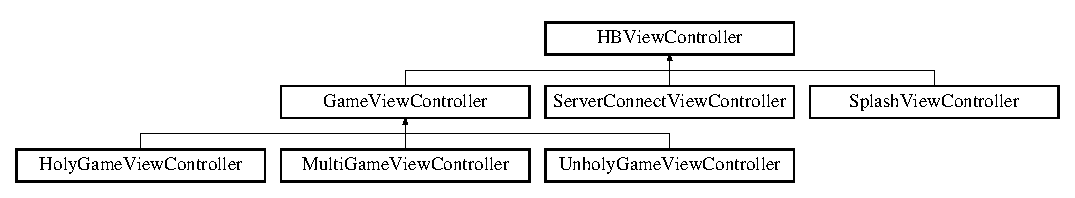
\includegraphics[height=2.210526cm]{class_h_b_view_controller}
\end{center}
\end{figure}
\subsection*{Public Member Functions}
\begin{DoxyCompactItemize}
\item 
\hypertarget{class_h_b_view_controller_ae5dce786709a034b56dc893bcc27a52e}{virtual H\-B\-View\-Mode {\bfseries did\-Finish\-View} ()=0}\label{class_h_b_view_controller_ae5dce786709a034b56dc893bcc27a52e}

\item 
\hypertarget{class_h_b_view_controller_a035724c01b98fdfcce78ceffc43a0b17}{virtual void {\bfseries process} ()=0}\label{class_h_b_view_controller_a035724c01b98fdfcce78ceffc43a0b17}

\item 
\hypertarget{class_h_b_view_controller_a1e99289ebec388efc9320866019ef101}{virtual void {\bfseries render} ()=0}\label{class_h_b_view_controller_a1e99289ebec388efc9320866019ef101}

\item 
\hypertarget{class_h_b_view_controller_ac247f604ad8e355e86d93157be4ea7a4}{virtual bool {\bfseries quit} ()=0}\label{class_h_b_view_controller_ac247f604ad8e355e86d93157be4ea7a4}

\end{DoxyCompactItemize}


The documentation for this class was generated from the following file\-:\begin{DoxyCompactItemize}
\item 
H\-B\-View\-Controller.\-h\end{DoxyCompactItemize}

\hypertarget{class_holy_game_view_controller}{\section{Holy\-Game\-View\-Controller Class Reference}
\label{class_holy_game_view_controller}\index{Holy\-Game\-View\-Controller@{Holy\-Game\-View\-Controller}}
}
Inheritance diagram for Holy\-Game\-View\-Controller\-:\begin{figure}[H]
\begin{center}
\leavevmode
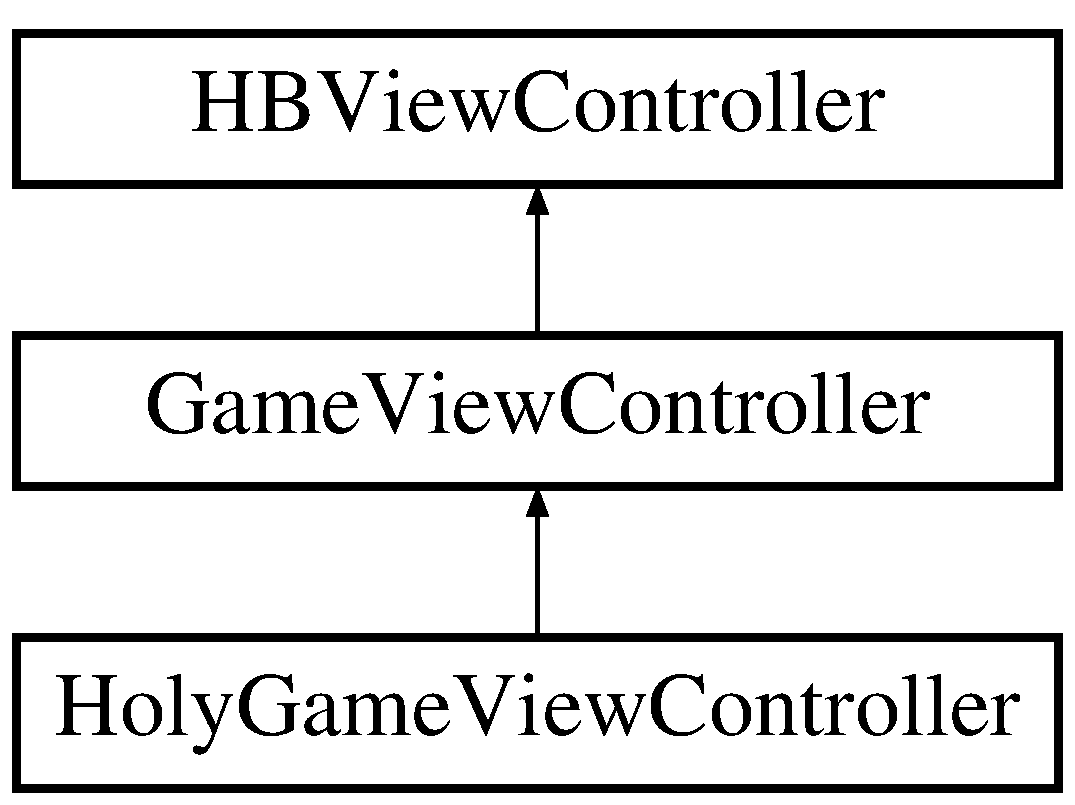
\includegraphics[height=3.000000cm]{class_holy_game_view_controller}
\end{center}
\end{figure}
\subsection*{Public Member Functions}
\begin{DoxyCompactItemize}
\item 
\hypertarget{class_holy_game_view_controller_a609559ed499e5d3c4c5102452efc1738}{void {\bfseries process} ()}\label{class_holy_game_view_controller_a609559ed499e5d3c4c5102452efc1738}

\item 
\hypertarget{class_holy_game_view_controller_a064f29bea316aa63bc5399419e1f356a}{void {\bfseries render} ()}\label{class_holy_game_view_controller_a064f29bea316aa63bc5399419e1f356a}

\end{DoxyCompactItemize}


The documentation for this class was generated from the following files\-:\begin{DoxyCompactItemize}
\item 
Holy\-Game\-View\-Controller.\-h\item 
Holy\-Game\-View\-Controller.\-cpp\end{DoxyCompactItemize}

\hypertarget{classinputmenuitem}{\section{inputmenuitem Class Reference}
\label{classinputmenuitem}\index{inputmenuitem@{inputmenuitem}}
}
Inheritance diagram for inputmenuitem\-:\begin{figure}[H]
\begin{center}
\leavevmode
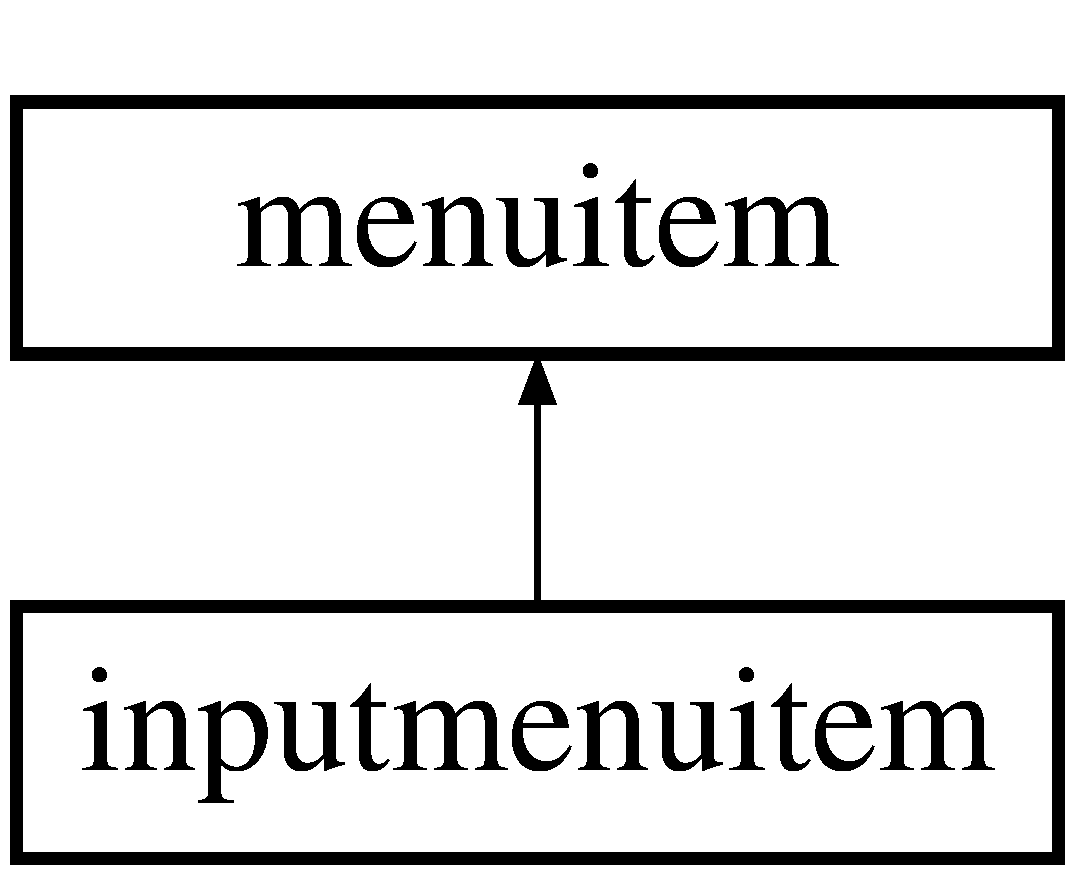
\includegraphics[height=2.000000cm]{classinputmenuitem}
\end{center}
\end{figure}
\subsection*{Public Member Functions}
\begin{DoxyCompactItemize}
\item 
\hypertarget{classinputmenuitem_a98392bce22539a262660d9af8ac54dc1}{{\footnotesize template$<$class A $>$ }\\{\bfseries inputmenuitem} (int max\-Input\-Len, A input\-Validator, char $\ast$init\-Input, char $\ast$iie, char $\ast$t, char $\ast$nam)}\label{classinputmenuitem_a98392bce22539a262660d9af8ac54dc1}

\item 
\hypertarget{classinputmenuitem_a04a64f8773fd62f74ff83005131221ef}{virtual bool {\bfseries activate} ()}\label{classinputmenuitem_a04a64f8773fd62f74ff83005131221ef}

\item 
\hypertarget{classinputmenuitem_a4cf096ba35175b1449f0e520b782c962}{virtual bool {\bfseries key\-\_\-input} (int key)}\label{classinputmenuitem_a4cf096ba35175b1449f0e520b782c962}

\item 
\hypertarget{classinputmenuitem_a51cbcdd67c8b4b1141f5fef1ac6674b1}{virtual void {\bfseries draw\-As\-Active} (unsigned char alpha)}\label{classinputmenuitem_a51cbcdd67c8b4b1141f5fef1ac6674b1}

\item 
\hypertarget{classinputmenuitem_a6761537bcc892dbcc772e45da3c7626d}{virtual bool {\bfseries should\-Menu\-Be\-Drawn} ()}\label{classinputmenuitem_a6761537bcc892dbcc772e45da3c7626d}

\item 
\hypertarget{classinputmenuitem_a272f77ba61bb730ca7e171e7ac148c50}{char $\ast$ {\bfseries get\-\_\-input} ()}\label{classinputmenuitem_a272f77ba61bb730ca7e171e7ac148c50}

\end{DoxyCompactItemize}


The documentation for this class was generated from the following files\-:\begin{DoxyCompactItemize}
\item 
menu.\-h\item 
menudraw.\-cpp\item 
menuitem.\-cpp\end{DoxyCompactItemize}

\hypertarget{classleavefunc}{\section{leavefunc Class Reference}
\label{classleavefunc}\index{leavefunc@{leavefunc}}
}
\subsection*{Public Member Functions}
\begin{DoxyCompactItemize}
\item 
\hypertarget{classleavefunc_a3945bc2bf6c7a6e20f63aa0d404539ef}{{\bfseries leavefunc} (\hyperlink{class_game_view_controller}{Game\-View\-Controller} $\ast$gvc)}\label{classleavefunc_a3945bc2bf6c7a6e20f63aa0d404539ef}

\item 
\hypertarget{classleavefunc_ad949ff1d0de1a12980191427bbde51e8}{bool {\bfseries operator()} (\hyperlink{structvoidtype}{voidtype})}\label{classleavefunc_ad949ff1d0de1a12980191427bbde51e8}

\end{DoxyCompactItemize}
\subsection*{Public Attributes}
\begin{DoxyCompactItemize}
\item 
\hypertarget{classleavefunc_a5c398672fa2a118d2c97af2296e20da6}{\hyperlink{class_game_view_controller}{Game\-View\-Controller} $\ast$ {\bfseries \-\_\-gvc}}\label{classleavefunc_a5c398672fa2a118d2c97af2296e20da6}

\end{DoxyCompactItemize}


The documentation for this class was generated from the following file\-:\begin{DoxyCompactItemize}
\item 
Game\-View\-Controller.\-h\end{DoxyCompactItemize}

\hypertarget{class_light}{\section{Light Class Reference}
\label{class_light}\index{Light@{Light}}
}
\subsection*{Public Attributes}
\begin{DoxyCompactItemize}
\item 
\hypertarget{class_light_a3a4fe35c2d1ce18e97c51ace85e2bcd0}{\hyperlink{class_vector3_d}{Vector3\-D} {\bfseries position}}\label{class_light_a3a4fe35c2d1ce18e97c51ace85e2bcd0}

\item 
\hypertarget{class_light_ad7a168d26aed1bf7cca1a8d8e6f8ada4}{\hyperlink{class_color}{Color} {\bfseries color}}\label{class_light_ad7a168d26aed1bf7cca1a8d8e6f8ada4}

\end{DoxyCompactItemize}


The documentation for this class was generated from the following file\-:\begin{DoxyCompactItemize}
\item 
hack.\-h\end{DoxyCompactItemize}

\hypertarget{class_material}{\section{Material Class Reference}
\label{class_material}\index{Material@{Material}}
}
Inheritance diagram for Material\-:\begin{figure}[H]
\begin{center}
\leavevmode
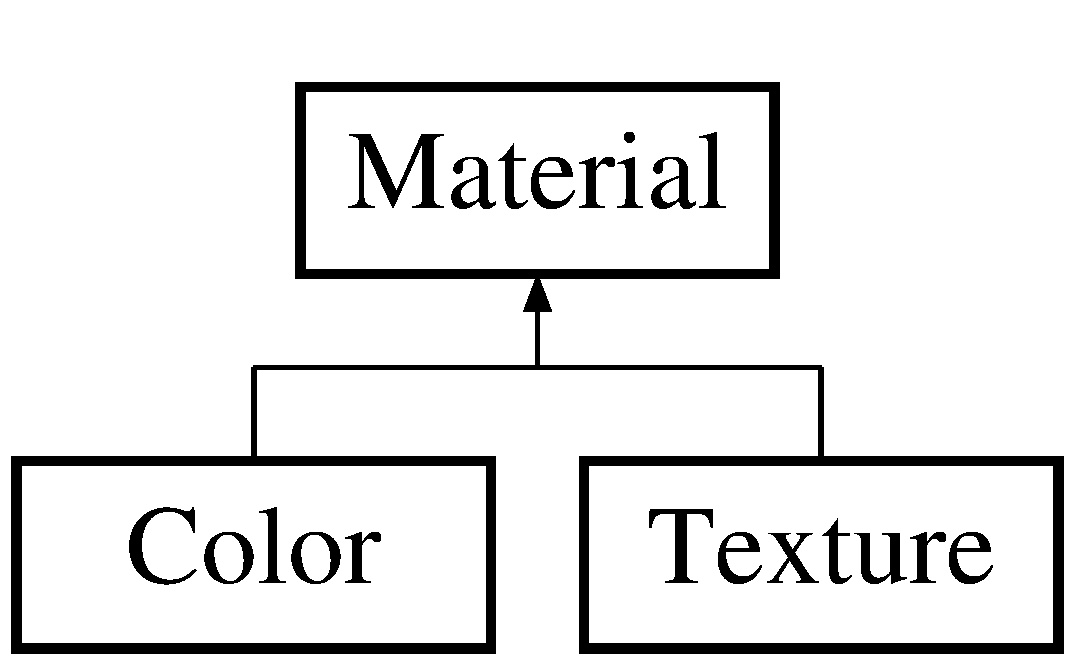
\includegraphics[height=2.000000cm]{class_material}
\end{center}
\end{figure}


The documentation for this class was generated from the following file\-:\begin{DoxyCompactItemize}
\item 
Material.\-h\end{DoxyCompactItemize}

\hypertarget{classmenu}{\section{menu Class Reference}
\label{classmenu}\index{menu@{menu}}
}
\subsection*{Public Member Functions}
\begin{DoxyCompactItemize}
\item 
\hypertarget{classmenu_a249a216b0c4fc43c605f5ee1cc6efdf0}{void {\bfseries add\-\_\-menuitem} (\hyperlink{classmenuitem}{menuitem} $\ast$a)}\label{classmenu_a249a216b0c4fc43c605f5ee1cc6efdf0}

\item 
\hypertarget{classmenu_ad127a885a2e996ba10d626d6feab7039}{void {\bfseries key\-\_\-input} (int key)}\label{classmenu_ad127a885a2e996ba10d626d6feab7039}

\item 
\hypertarget{classmenu_a66972e75031e55aca63a973e67f5a82b}{bool {\bfseries is\-\_\-active} ()}\label{classmenu_a66972e75031e55aca63a973e67f5a82b}

\item 
\hypertarget{classmenu_af1697c138773f4d23f73f042f49aade5}{void {\bfseries set\-\_\-active} (bool)}\label{classmenu_af1697c138773f4d23f73f042f49aade5}

\item 
\hypertarget{classmenu_a6fcf97a34d06d1889ae8cf52e5060d06}{void {\bfseries draw} ()}\label{classmenu_a6fcf97a34d06d1889ae8cf52e5060d06}

\item 
\hypertarget{classmenu_ae817e5dae0bb7b87f979aff7e3b07cb9}{void {\bfseries draw\-Menu} ()}\label{classmenu_ae817e5dae0bb7b87f979aff7e3b07cb9}

\item 
\hypertarget{classmenu_a80c0c04f4a6569cdc7f6161139570eb2}{void {\bfseries set\-Appearance} (bool transparent, float x1, float x2, float y1, float y2)}\label{classmenu_a80c0c04f4a6569cdc7f6161139570eb2}

\item 
\hypertarget{classmenu_ad4331a050513af4f341120c1533856f2}{void {\bfseries set\-Appearance\-Full} ()}\label{classmenu_ad4331a050513af4f341120c1533856f2}

\item 
\hypertarget{classmenu_a4e1f99eb6b363998f6f54cf444729422}{void {\bfseries set\-Appearance\-Middle} ()}\label{classmenu_a4e1f99eb6b363998f6f54cf444729422}

\end{DoxyCompactItemize}


The documentation for this class was generated from the following files\-:\begin{DoxyCompactItemize}
\item 
menu.\-h\item 
menu.\-cpp\item 
menudraw.\-cpp\end{DoxyCompactItemize}

\hypertarget{classmenuitem}{\section{menuitem Class Reference}
\label{classmenuitem}\index{menuitem@{menuitem}}
}
Inheritance diagram for menuitem\-:\begin{figure}[H]
\begin{center}
\leavevmode
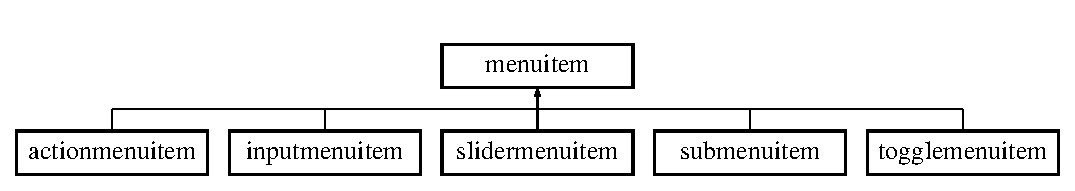
\includegraphics[height=2.000000cm]{classmenuitem}
\end{center}
\end{figure}
\subsection*{Public Member Functions}
\begin{DoxyCompactItemize}
\item 
\hypertarget{classmenuitem_a1cd433f71ec87a82e02bc105d4bcde13}{virtual bool {\bfseries activate} ()}\label{classmenuitem_a1cd433f71ec87a82e02bc105d4bcde13}

\item 
\hypertarget{classmenuitem_a67852d94fa74d5b75cfff6fbd0f113cb}{virtual bool {\bfseries key\-\_\-input} (int key)}\label{classmenuitem_a67852d94fa74d5b75cfff6fbd0f113cb}

\item 
\hypertarget{classmenuitem_a85a5989ec80f92cd77c6f91b4e57a1e7}{virtual void {\bfseries key\-\_\-input\-\_\-non\-\_\-active} (int key)}\label{classmenuitem_a85a5989ec80f92cd77c6f91b4e57a1e7}

\item 
\hypertarget{classmenuitem_a1398cc7e99754db2824bcd0a310901d2}{virtual void {\bfseries draw} (bool selected, float x1, float y1, float width, float height, unsigned char alpha)}\label{classmenuitem_a1398cc7e99754db2824bcd0a310901d2}

\item 
\hypertarget{classmenuitem_aeb0cc4c1f6632df5e3e70e53d68b5641}{virtual void {\bfseries draw\-As\-Active} (unsigned char alpha)}\label{classmenuitem_aeb0cc4c1f6632df5e3e70e53d68b5641}

\item 
\hypertarget{classmenuitem_ae6d98769321752ff844e5e566f614098}{virtual bool {\bfseries should\-Menu\-Be\-Drawn} ()}\label{classmenuitem_ae6d98769321752ff844e5e566f614098}

\item 
\hypertarget{classmenuitem_a247b8c4cc76430523f69f5c1b47c0c91}{virtual void {\bfseries on\-Select} ()}\label{classmenuitem_a247b8c4cc76430523f69f5c1b47c0c91}

\item 
\hypertarget{classmenuitem_ae59b15770dbdcfad2f96ca9e610e2726}{virtual void {\bfseries on\-Deselect} ()}\label{classmenuitem_ae59b15770dbdcfad2f96ca9e610e2726}

\end{DoxyCompactItemize}
\subsection*{Protected Attributes}
\begin{DoxyCompactItemize}
\item 
\hypertarget{classmenuitem_a8b41220a5636c9fb902efbf7499e18f0}{char $\ast$ {\bfseries name}}\label{classmenuitem_a8b41220a5636c9fb902efbf7499e18f0}

\end{DoxyCompactItemize}


The documentation for this class was generated from the following files\-:\begin{DoxyCompactItemize}
\item 
menu.\-h\item 
menudraw.\-cpp\item 
menuitem.\-cpp\end{DoxyCompactItemize}

\hypertarget{class_multi_game_view_controller}{\section{Multi\-Game\-View\-Controller Class Reference}
\label{class_multi_game_view_controller}\index{Multi\-Game\-View\-Controller@{Multi\-Game\-View\-Controller}}
}
Inheritance diagram for Multi\-Game\-View\-Controller\-:\begin{figure}[H]
\begin{center}
\leavevmode
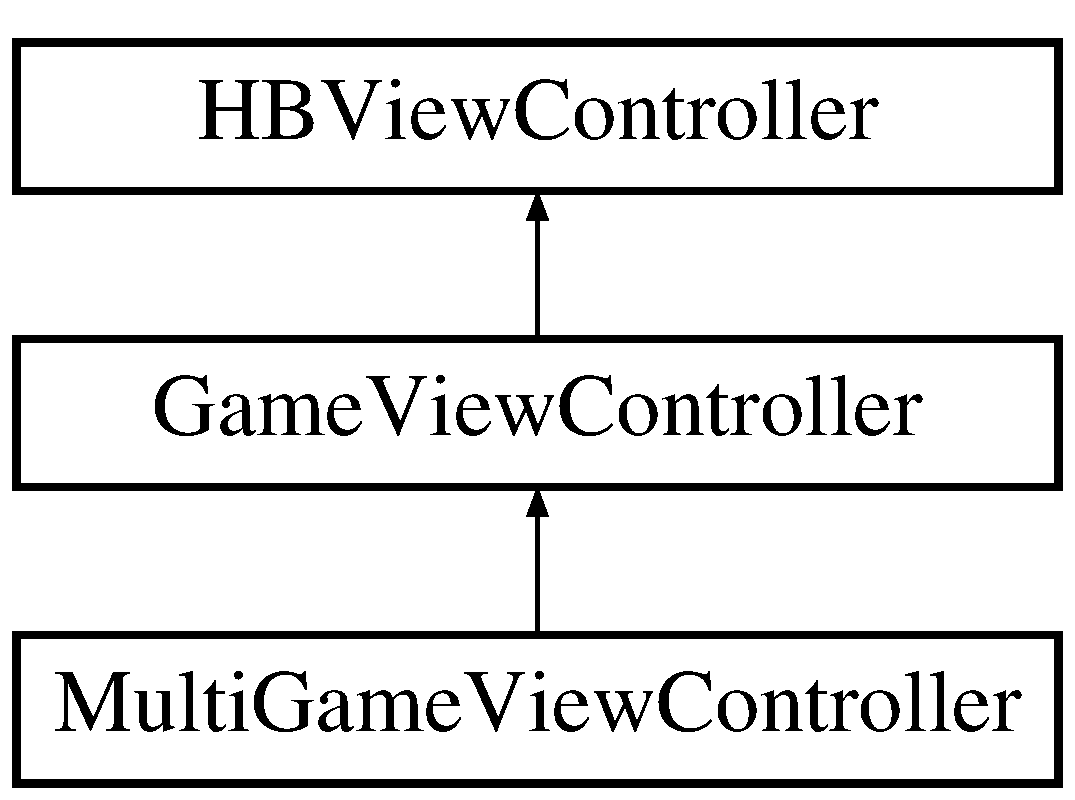
\includegraphics[height=3.000000cm]{class_multi_game_view_controller}
\end{center}
\end{figure}
\subsection*{Public Member Functions}
\begin{DoxyCompactItemize}
\item 
\hypertarget{class_multi_game_view_controller_a3c8f554d074bd4182181d093ce1fe1d6}{void {\bfseries process} ()}\label{class_multi_game_view_controller_a3c8f554d074bd4182181d093ce1fe1d6}

\item 
\hypertarget{class_multi_game_view_controller_ac2a0388681043469fba5ec4722e5d7ef}{void {\bfseries render} ()}\label{class_multi_game_view_controller_ac2a0388681043469fba5ec4722e5d7ef}

\end{DoxyCompactItemize}


The documentation for this class was generated from the following files\-:\begin{DoxyCompactItemize}
\item 
Multi\-Game\-View\-Controller.\-h\item 
Multi\-Game\-View\-Controller.\-cpp\end{DoxyCompactItemize}

\hypertarget{class_object}{\section{Object Class Reference}
\label{class_object}\index{Object@{Object}}
}
\subsection*{Public Member Functions}
\begin{DoxyCompactItemize}
\item 
\hypertarget{class_object_a9b9c9d7a76b1dae92f07c51181513ca4}{void {\bfseries write\-\_\-data} (\hyperlink{class_write_packet}{Write\-Packet} $\ast$wp)}\label{class_object_a9b9c9d7a76b1dae92f07c51181513ca4}

\item 
\hypertarget{class_object_a38c8d7375c607ed8c60c7a21c1dfc21d}{void {\bfseries read\-\_\-data} (\hyperlink{class_read_packet}{Read\-Packet} $\ast$rp)}\label{class_object_a38c8d7375c607ed8c60c7a21c1dfc21d}

\end{DoxyCompactItemize}
\subsection*{Public Attributes}
\begin{DoxyCompactItemize}
\item 
\hypertarget{class_object_a99f124fb1348ce54003a170411919913}{\hyperlink{class_vector2_d}{Vector2\-D} {\bfseries p}}\label{class_object_a99f124fb1348ce54003a170411919913}

\item 
\hypertarget{class_object_a08dada56e9bde8cbda508c7fb1bae00b}{\hyperlink{class_vector2_d}{Vector2\-D} {\bfseries v}}\label{class_object_a08dada56e9bde8cbda508c7fb1bae00b}

\item 
\hypertarget{class_object_a60866179af7cb2aad410ea01de546e4e}{float {\bfseries mass}}\label{class_object_a60866179af7cb2aad410ea01de546e4e}

\item 
\hypertarget{class_object_a78dfb0ff4a8ea85a6de266cc1ebff93a}{float {\bfseries rad}}\label{class_object_a78dfb0ff4a8ea85a6de266cc1ebff93a}

\item 
\hypertarget{class_object_a3ed85d6e0b0b62ff2501d421cb55c5e9}{\hyperlink{class_color}{Color} {\bfseries color}}\label{class_object_a3ed85d6e0b0b62ff2501d421cb55c5e9}

\item 
\hypertarget{class_object_acdb5ddc034cf35c452c2f5cfcbf8c0e4}{float {\bfseries hrat}}\label{class_object_acdb5ddc034cf35c452c2f5cfcbf8c0e4}

\item 
\hypertarget{class_object_aa7caf12457afb8b79152cfaf0158c827}{int {\bfseries id}}\label{class_object_aa7caf12457afb8b79152cfaf0158c827}

\item 
\hypertarget{class_object_a3b1f27788974d367db00ea4e87873d1d}{bool {\bfseries dead}}\label{class_object_a3b1f27788974d367db00ea4e87873d1d}

\item 
\hypertarget{class_object_a8ef3a022a1544f35c79d79b3f61fcbb1}{bool {\bfseries stopped}}\label{class_object_a8ef3a022a1544f35c79d79b3f61fcbb1}

\item 
\hypertarget{class_object_ab39618b61cf21a25135a5b08a8a51a95}{int {\bfseries spawnl}}\label{class_object_ab39618b61cf21a25135a5b08a8a51a95}

\item 
\hypertarget{class_object_a962a545cf1ba17dc15f2d08b2012d968}{int {\bfseries spawny}}\label{class_object_a962a545cf1ba17dc15f2d08b2012d968}

\item 
\hypertarget{class_object_aed601a91f4458261950570d45e5c368f}{double {\bfseries time\-\_\-until\-\_\-spawn}}\label{class_object_aed601a91f4458261950570d45e5c368f}

\item 
\hypertarget{class_object_af0f3383d9cefc68ed8d68207c0972805}{int {\bfseries nattached}}\label{class_object_af0f3383d9cefc68ed8d68207c0972805}

\item 
\hypertarget{class_object_aad5e8ce72a70aa847afde2f496c69b53}{int {\bfseries attached\-To}}\label{class_object_aad5e8ce72a70aa847afde2f496c69b53}

\item 
\hypertarget{class_object_a8e4e31b38cc34a9b0eb8453f5151412f}{int {\bfseries player}}\label{class_object_a8e4e31b38cc34a9b0eb8453f5151412f}

\item 
\hypertarget{class_object_ab51b11311d5cc603dea0a86960512cd7}{int {\bfseries flag}}\label{class_object_ab51b11311d5cc603dea0a86960512cd7}

\end{DoxyCompactItemize}


The documentation for this class was generated from the following files\-:\begin{DoxyCompactItemize}
\item 
hack.\-h\item 
object.\-cpp\end{DoxyCompactItemize}

\hypertarget{class_obstacle}{\section{Obstacle Class Reference}
\label{class_obstacle}\index{Obstacle@{Obstacle}}
}
\subsection*{Public Member Functions}
\begin{DoxyCompactItemize}
\item 
\hypertarget{class_obstacle_ab700c6e78d18d2a2b624a65c50e79b2d}{{\bfseries Obstacle} (\hyperlink{class_vector2_d}{Vector2\-D} a, \hyperlink{class_vector2_d}{Vector2\-D} b, \hyperlink{class_color}{Color} c, Wall\-Type d, int e=N\-O\-\_\-\-T\-E\-A\-M)}\label{class_obstacle_ab700c6e78d18d2a2b624a65c50e79b2d}

\end{DoxyCompactItemize}
\subsection*{Public Attributes}
\begin{DoxyCompactItemize}
\item 
\hypertarget{class_obstacle_ab8a54c75f67fcd88623131d45e0589b2}{\hyperlink{class_vector2_d}{Vector2\-D} {\bfseries p1}}\label{class_obstacle_ab8a54c75f67fcd88623131d45e0589b2}

\item 
\hypertarget{class_obstacle_a4c453b0020f3b3f09052082e6b87de48}{\hyperlink{class_vector2_d}{Vector2\-D} {\bfseries p2}}\label{class_obstacle_a4c453b0020f3b3f09052082e6b87de48}

\item 
\hypertarget{class_obstacle_ab5b698fc36de4c1e15730219ddd579c9}{\hyperlink{class_color}{Color} {\bfseries color}}\label{class_obstacle_ab5b698fc36de4c1e15730219ddd579c9}

\item 
\hypertarget{class_obstacle_aded042e99ff96538f3d4aa70a1da25ba}{bool {\bfseries sticky}}\label{class_obstacle_aded042e99ff96538f3d4aa70a1da25ba}

\item 
\hypertarget{class_obstacle_a041170d3a6a105eb72e94b821dbea239}{int {\bfseries flag}}\label{class_obstacle_a041170d3a6a105eb72e94b821dbea239}

\item 
\hypertarget{class_obstacle_abb6983458bd420b3e2f8fde6000c308a}{Wall\-Type {\bfseries wall\-Type}}\label{class_obstacle_abb6983458bd420b3e2f8fde6000c308a}

\end{DoxyCompactItemize}


The documentation for this class was generated from the following file\-:\begin{DoxyCompactItemize}
\item 
hack.\-h\end{DoxyCompactItemize}

\hypertarget{class_parse_exception}{\section{Parse\-Exception Class Reference}
\label{class_parse_exception}\index{Parse\-Exception@{Parse\-Exception}}
}
\subsection*{Public Member Functions}
\begin{DoxyCompactItemize}
\item 
\hypertarget{class_parse_exception_ae42a372f3acb960331402fcca1808b52}{{\bfseries Parse\-Exception} (std\-::string msg=\char`\"{}\char`\"{})}\label{class_parse_exception_ae42a372f3acb960331402fcca1808b52}

\item 
\hypertarget{class_parse_exception_a3325238091196c8b7b48475734850f83}{const char $\ast$ {\bfseries what} () const   throw ()}\label{class_parse_exception_a3325238091196c8b7b48475734850f83}

\end{DoxyCompactItemize}


The documentation for this class was generated from the following file\-:\begin{DoxyCompactItemize}
\item 
H\-B\-Map.\-cpp\end{DoxyCompactItemize}

\hypertarget{class_player}{\section{Player Class Reference}
\label{class_player}\index{Player@{Player}}
}
\subsection*{Public Attributes}
\begin{DoxyCompactItemize}
\item 
\hypertarget{class_player_a22c96380052d528c6e0eec91ceaf334b}{\hyperlink{class_client}{Client} {\bfseries cl}}\label{class_player_a22c96380052d528c6e0eec91ceaf334b}

\item 
\hypertarget{class_player_a8cb531195e9d96c8320cfbe0fc145495}{int {\bfseries object\-\_\-id}}\label{class_player_a8cb531195e9d96c8320cfbe0fc145495}

\item 
\hypertarget{class_player_ab5e831cac1c83f718e1dfa72aba77d06}{char {\bfseries key\-\_\-pressed}}\label{class_player_ab5e831cac1c83f718e1dfa72aba77d06}

\item 
\hypertarget{class_player_acdf217201e6fe6ed898c2e15292ef252}{float {\bfseries angle}}\label{class_player_acdf217201e6fe6ed898c2e15292ef252}

\item 
\hypertarget{class_player_ad29b77b310b9417af5ded0fe08778ac3}{double {\bfseries time\-\_\-until\-\_\-spawn}}\label{class_player_ad29b77b310b9417af5ded0fe08778ac3}

\item 
\hypertarget{class_player_a26731f05ed89c4f8a30ec960d217d746}{int {\bfseries team}}\label{class_player_a26731f05ed89c4f8a30ec960d217d746}

\end{DoxyCompactItemize}


The documentation for this class was generated from the following file\-:\begin{DoxyCompactItemize}
\item 
game.\-h\end{DoxyCompactItemize}

\hypertarget{classquitfunc}{\section{quitfunc Class Reference}
\label{classquitfunc}\index{quitfunc@{quitfunc}}
}
\subsection*{Public Member Functions}
\begin{DoxyCompactItemize}
\item 
\hypertarget{classquitfunc_a92ee5f3eaa036a45ff2e1efe731ed0fe}{{\bfseries quitfunc} (\hyperlink{class_h_b_view_controller}{H\-B\-View\-Controller} $\ast$vc)}\label{classquitfunc_a92ee5f3eaa036a45ff2e1efe731ed0fe}

\item 
\hypertarget{classquitfunc_af8642bda915f28bcbfff712ddaa8c519}{bool {\bfseries operator()} (\hyperlink{structvoidtype}{voidtype})}\label{classquitfunc_af8642bda915f28bcbfff712ddaa8c519}

\end{DoxyCompactItemize}
\subsection*{Public Attributes}
\begin{DoxyCompactItemize}
\item 
\hypertarget{classquitfunc_a1bd7c289906407c0015772194704ab1b}{\hyperlink{class_h_b_view_controller}{H\-B\-View\-Controller} $\ast$ {\bfseries \-\_\-vc}}\label{classquitfunc_a1bd7c289906407c0015772194704ab1b}

\end{DoxyCompactItemize}


The documentation for this class was generated from the following file\-:\begin{DoxyCompactItemize}
\item 
menufuncs.\-h\end{DoxyCompactItemize}

\hypertarget{class_read_packet}{\section{Read\-Packet Class Reference}
\label{class_read_packet}\index{Read\-Packet@{Read\-Packet}}
}
\subsection*{Public Member Functions}
\begin{DoxyCompactItemize}
\item 
\hypertarget{class_read_packet_a00a7b6a89da284df88ca3f8ab55fae2d}{{\bfseries Read\-Packet} (char message\-\_\-type, int size, int packet\-\_\-number)}\label{class_read_packet_a00a7b6a89da284df88ca3f8ab55fae2d}

\item 
\hypertarget{class_read_packet_a63753af52ef533c66b3be50872f3abd2}{char {\bfseries read\-\_\-char} ()}\label{class_read_packet_a63753af52ef533c66b3be50872f3abd2}

\item 
\hypertarget{class_read_packet_ad8d4bb0fe52c7660db0cd089fd2e5c4a}{int {\bfseries read\-\_\-int} ()}\label{class_read_packet_ad8d4bb0fe52c7660db0cd089fd2e5c4a}

\item 
\hypertarget{class_read_packet_a63f15fc734db95aaa4ab56938ff94baf}{short {\bfseries read\-\_\-short} ()}\label{class_read_packet_a63f15fc734db95aaa4ab56938ff94baf}

\item 
\hypertarget{class_read_packet_a7d91d8e037415dc26ec105175bc6de6a}{float {\bfseries read\-\_\-float} ()}\label{class_read_packet_a7d91d8e037415dc26ec105175bc6de6a}

\item 
\hypertarget{class_read_packet_ae69e582fd3c4408b44b686e2707fdee8}{std\-::string {\bfseries read\-\_\-string} ()}\label{class_read_packet_ae69e582fd3c4408b44b686e2707fdee8}

\end{DoxyCompactItemize}
\subsection*{Public Attributes}
\begin{DoxyCompactItemize}
\item 
\hypertarget{class_read_packet_afc99f7f5987ddc435d8bea3cad22183a}{int {\bfseries size}}\label{class_read_packet_afc99f7f5987ddc435d8bea3cad22183a}

\item 
\hypertarget{class_read_packet_a3547d75436b725e96ac698be40756af2}{char $\ast$ {\bfseries buf}}\label{class_read_packet_a3547d75436b725e96ac698be40756af2}

\item 
\hypertarget{class_read_packet_a0e5874d215ddcb1c9ece48229f4bca22}{char {\bfseries message\-\_\-type}}\label{class_read_packet_a0e5874d215ddcb1c9ece48229f4bca22}

\item 
\hypertarget{class_read_packet_acbe782b102a78ad0238daa933306f3b5}{int {\bfseries index}}\label{class_read_packet_acbe782b102a78ad0238daa933306f3b5}

\item 
\hypertarget{class_read_packet_a548c347871c323ffae1cc037e5923f72}{int {\bfseries packet\-\_\-number}}\label{class_read_packet_a548c347871c323ffae1cc037e5923f72}

\end{DoxyCompactItemize}


The documentation for this class was generated from the following files\-:\begin{DoxyCompactItemize}
\item 
packet.\-h\item 
packet.\-cpp\end{DoxyCompactItemize}

\hypertarget{class_rectangular_object}{\section{Rectangular\-Object Class Reference}
\label{class_rectangular_object}\index{Rectangular\-Object@{Rectangular\-Object}}
}
Inheritance diagram for Rectangular\-Object\-:\begin{figure}[H]
\begin{center}
\leavevmode
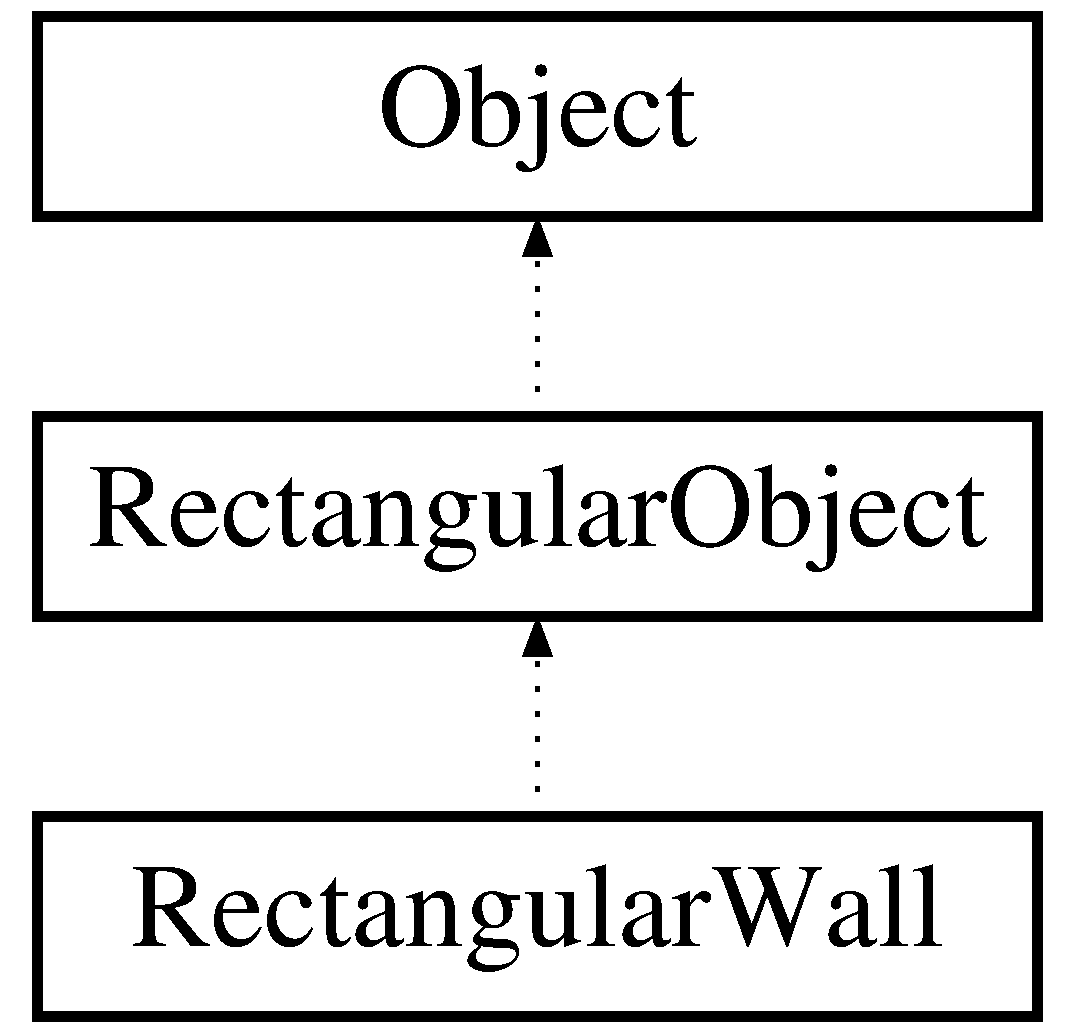
\includegraphics[height=3.000000cm]{class_rectangular_object}
\end{center}
\end{figure}
\subsection*{Public Member Functions}
\begin{DoxyCompactItemize}
\item 
\hyperlink{class_rectangular_object_ac72890aadfeaa97e69b7ae86a327ea62}{Rectangular\-Object} (\hyperlink{class_vector2_d}{Vector2\-D} a, \hyperlink{class_vector2_d}{Vector2\-D} b, \hyperlink{class_material}{Material} m)
\item 
const \hyperlink{class_vector2_d}{Vector2\-D} \& \hyperlink{class_rectangular_object_ae6270bd7cae4656af857dd9eaa043137}{get\-P1} () const 
\item 
const \hyperlink{class_vector2_d}{Vector2\-D} \& \hyperlink{class_rectangular_object_a184eb6a812597ab9761b4307aa3e85e3}{get\-P2} () const 
\end{DoxyCompactItemize}


\subsection{Constructor \& Destructor Documentation}
\hypertarget{class_rectangular_object_ac72890aadfeaa97e69b7ae86a327ea62}{\index{Rectangular\-Object@{Rectangular\-Object}!Rectangular\-Object@{Rectangular\-Object}}
\index{Rectangular\-Object@{Rectangular\-Object}!RectangularObject@{Rectangular\-Object}}
\subsubsection[{Rectangular\-Object}]{\setlength{\rightskip}{0pt plus 5cm}{\bf Rectangular\-Object\-::\-Rectangular\-Object} (
\begin{DoxyParamCaption}
\item[{{\bf Vector2\-D}}]{a, }
\item[{{\bf Vector2\-D}}]{b, }
\item[{{\bf Material}}]{m}
\end{DoxyParamCaption}
)\hspace{0.3cm}{\ttfamily  \mbox{[}inline\mbox{]}}}}\label{class_rectangular_object_ac72890aadfeaa97e69b7ae86a327ea62}
Constructs a \hyperlink{class_rectangular_object}{Rectangular\-Object} between the given two points and with the given material. 
\begin{DoxyParams}{Parameters}
{\em a} & First endpoint of the wall. \\
\hline
{\em b} & Second endpoint of the wall. \\
\hline
{\em m} & The material for the object being created. \\
\hline
\end{DoxyParams}


\subsection{Member Function Documentation}
\hypertarget{class_rectangular_object_ae6270bd7cae4656af857dd9eaa043137}{\index{Rectangular\-Object@{Rectangular\-Object}!get\-P1@{get\-P1}}
\index{get\-P1@{get\-P1}!RectangularObject@{Rectangular\-Object}}
\subsubsection[{get\-P1}]{\setlength{\rightskip}{0pt plus 5cm}const {\bf Vector2\-D}\& {\bf Rectangular\-Object\-::get\-P1} (
\begin{DoxyParamCaption}
{}
\end{DoxyParamCaption}
) const\hspace{0.3cm}{\ttfamily  \mbox{[}inline\mbox{]}}}}\label{class_rectangular_object_ae6270bd7cae4656af857dd9eaa043137}
\begin{DoxyReturn}{Returns}
the first endpoint of the object 
\end{DoxyReturn}
\hypertarget{class_rectangular_object_a184eb6a812597ab9761b4307aa3e85e3}{\index{Rectangular\-Object@{Rectangular\-Object}!get\-P2@{get\-P2}}
\index{get\-P2@{get\-P2}!RectangularObject@{Rectangular\-Object}}
\subsubsection[{get\-P2}]{\setlength{\rightskip}{0pt plus 5cm}const {\bf Vector2\-D}\& {\bf Rectangular\-Object\-::get\-P2} (
\begin{DoxyParamCaption}
{}
\end{DoxyParamCaption}
) const\hspace{0.3cm}{\ttfamily  \mbox{[}inline\mbox{]}}}}\label{class_rectangular_object_a184eb6a812597ab9761b4307aa3e85e3}
\begin{DoxyReturn}{Returns}
the second endpoint of the object 
\end{DoxyReturn}


The documentation for this class was generated from the following file\-:\begin{DoxyCompactItemize}
\item 
Object.\-h\end{DoxyCompactItemize}

\hypertarget{class_rectangular_wall}{\section{Rectangular\-Wall Class Reference}
\label{class_rectangular_wall}\index{Rectangular\-Wall@{Rectangular\-Wall}}
}
Inheritance diagram for Rectangular\-Wall\-:\begin{figure}[H]
\begin{center}
\leavevmode
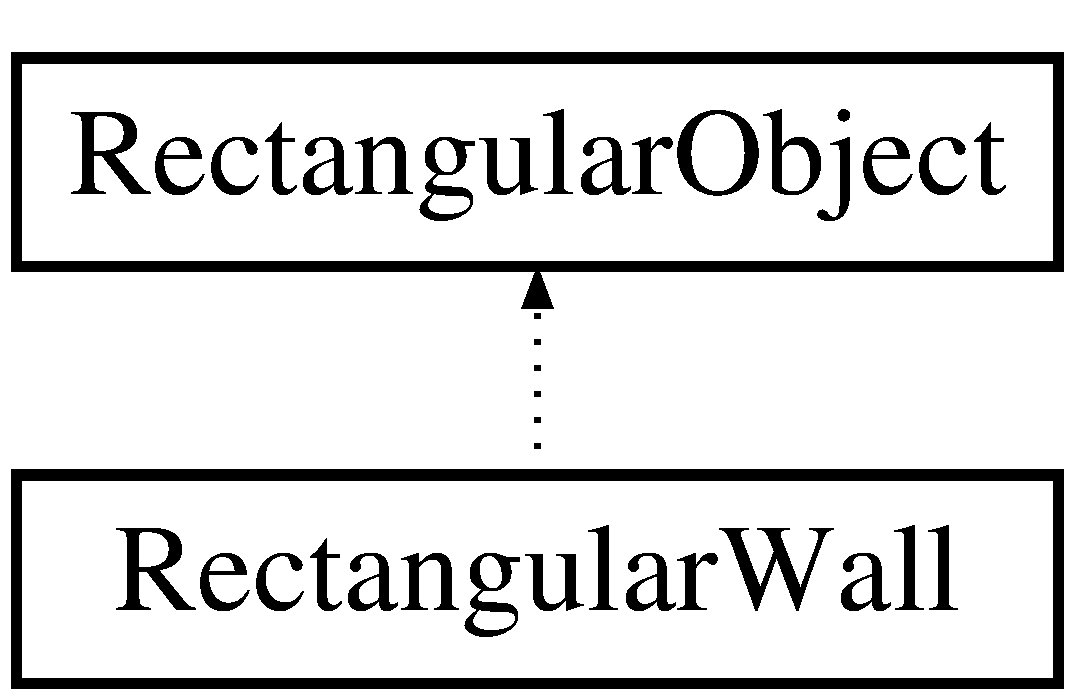
\includegraphics[height=2.000000cm]{class_rectangular_wall}
\end{center}
\end{figure}
\subsection*{Public Member Functions}
\begin{DoxyCompactItemize}
\item 
\hyperlink{class_rectangular_wall_a6bdc8ee8d5eab92ff3cd5c5ddfb3cec7}{Rectangular\-Wall} (\hyperlink{class_vector2_d}{Vector2\-D} a, \hyperlink{class_vector2_d}{Vector2\-D} b, \hyperlink{class_material}{Material} m, Wall\-Type wt=W\-T\-\_\-\-N\-O\-R\-M\-A\-L)
\item 
const Wall\-Type \& \hyperlink{class_rectangular_wall_addadf7e209644cb19781ba243740f1f3}{get\-Wall\-Type} () const 
\end{DoxyCompactItemize}


\subsection{Constructor \& Destructor Documentation}
\hypertarget{class_rectangular_wall_a6bdc8ee8d5eab92ff3cd5c5ddfb3cec7}{\index{Rectangular\-Wall@{Rectangular\-Wall}!Rectangular\-Wall@{Rectangular\-Wall}}
\index{Rectangular\-Wall@{Rectangular\-Wall}!RectangularWall@{Rectangular\-Wall}}
\subsubsection[{Rectangular\-Wall}]{\setlength{\rightskip}{0pt plus 5cm}{\bf Rectangular\-Wall\-::\-Rectangular\-Wall} (
\begin{DoxyParamCaption}
\item[{{\bf Vector2\-D}}]{a, }
\item[{{\bf Vector2\-D}}]{b, }
\item[{{\bf Material}}]{m, }
\item[{Wall\-Type}]{wt = {\ttfamily WT\-\_\-NORMAL}}
\end{DoxyParamCaption}
)\hspace{0.3cm}{\ttfamily  \mbox{[}inline\mbox{]}}}}\label{class_rectangular_wall_a6bdc8ee8d5eab92ff3cd5c5ddfb3cec7}
Constructs a \hyperlink{class_rectangular_wall}{Rectangular\-Wall} between the given two points and with the given material. 
\begin{DoxyParams}{Parameters}
{\em a} & First endpoint of the wall. \\
\hline
{\em b} & Second endpoint of the wall. \\
\hline
{\em m} & The material for the object being created. \\
\hline
\end{DoxyParams}


\subsection{Member Function Documentation}
\hypertarget{class_rectangular_wall_addadf7e209644cb19781ba243740f1f3}{\index{Rectangular\-Wall@{Rectangular\-Wall}!get\-Wall\-Type@{get\-Wall\-Type}}
\index{get\-Wall\-Type@{get\-Wall\-Type}!RectangularWall@{Rectangular\-Wall}}
\subsubsection[{get\-Wall\-Type}]{\setlength{\rightskip}{0pt plus 5cm}const Wall\-Type\& {\bf Rectangular\-Wall\-::get\-Wall\-Type} (
\begin{DoxyParamCaption}
{}
\end{DoxyParamCaption}
) const\hspace{0.3cm}{\ttfamily  \mbox{[}inline\mbox{]}}}}\label{class_rectangular_wall_addadf7e209644cb19781ba243740f1f3}
\begin{DoxyReturn}{Returns}
the wall type 
\end{DoxyReturn}


The documentation for this class was generated from the following file\-:\begin{DoxyCompactItemize}
\item 
Object.\-h\end{DoxyCompactItemize}

\hypertarget{class_round_object}{\section{Round\-Object Class Reference}
\label{class_round_object}\index{Round\-Object@{Round\-Object}}
}
Inheritance diagram for Round\-Object\-:\begin{figure}[H]
\begin{center}
\leavevmode
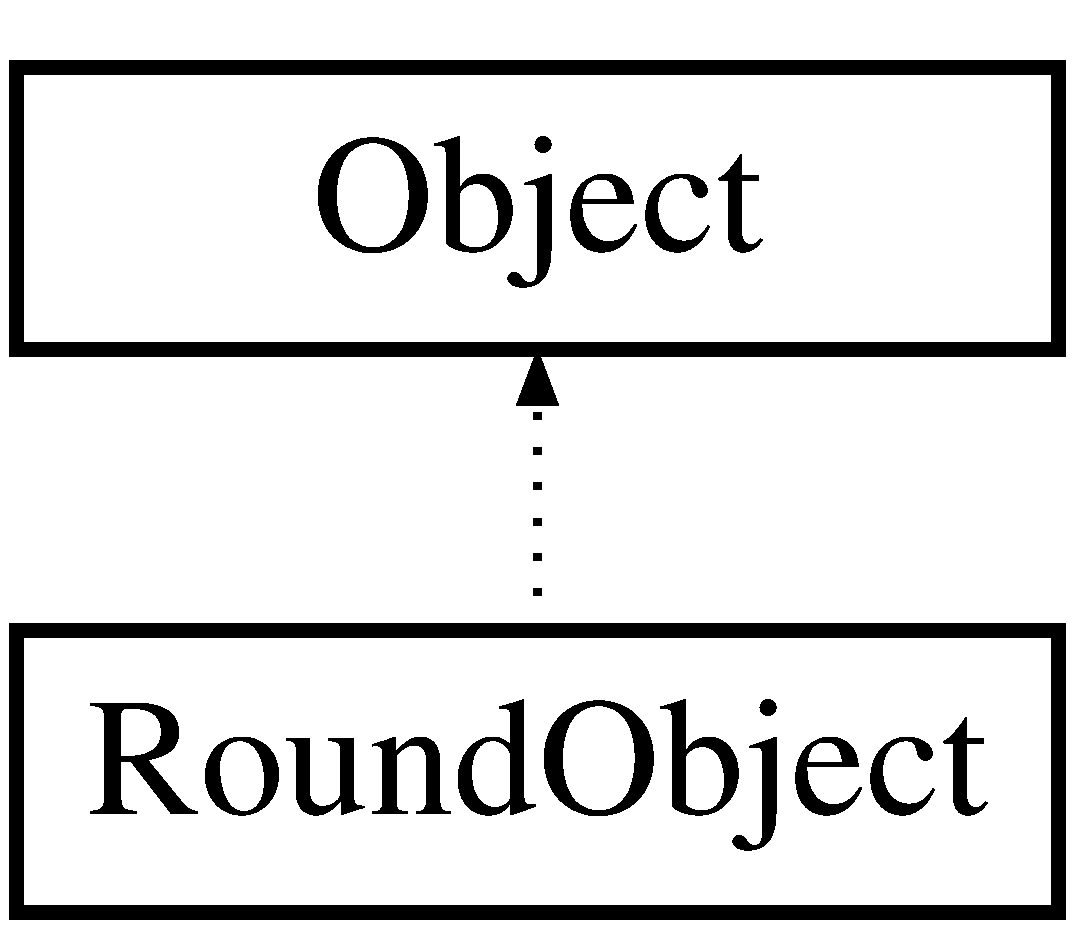
\includegraphics[height=2.000000cm]{class_round_object}
\end{center}
\end{figure}
\subsection*{Public Member Functions}
\begin{DoxyCompactItemize}
\item 
\hyperlink{class_round_object_a5ced474e09b2284b3d99380b2cd82d8f}{Round\-Object} (\hyperlink{class_material}{Material} material, \hyperlink{class_vector2_d}{Vector2\-D} center, float radius, float start\-Angle=0.\-0, float end\-Angle=M\-\_\-\-P\-I\-\_\-2)
\item 
const \hyperlink{class_vector2_d}{Vector2\-D} \& \hyperlink{class_round_object_a6998fa9d51ab4814ceb242df9e6031b5}{get\-Center} () const 
\item 
const float \& \hyperlink{class_round_object_a754405df28786cd80d50fe911dc220ca}{get\-Radius} () const 
\item 
const float \& \hyperlink{class_round_object_a748fc039f7a76a495c8ee51476d56df1}{get\-Start\-Angle} () const 
\item 
const float \& \hyperlink{class_round_object_a775ee05b5e644b07522dfb3654cfe114}{get\-End\-Angle} () const 
\end{DoxyCompactItemize}
\subsection*{Protected Attributes}
\begin{DoxyCompactItemize}
\item 
\hypertarget{class_round_object_a0a0b04b4676fc85d6e8f03f80541c8f6}{float {\bfseries center}}\label{class_round_object_a0a0b04b4676fc85d6e8f03f80541c8f6}

\end{DoxyCompactItemize}


\subsection{Constructor \& Destructor Documentation}
\hypertarget{class_round_object_a5ced474e09b2284b3d99380b2cd82d8f}{\index{Round\-Object@{Round\-Object}!Round\-Object@{Round\-Object}}
\index{Round\-Object@{Round\-Object}!RoundObject@{Round\-Object}}
\subsubsection[{Round\-Object}]{\setlength{\rightskip}{0pt plus 5cm}{\bf Round\-Object\-::\-Round\-Object} (
\begin{DoxyParamCaption}
\item[{{\bf Material}}]{material, }
\item[{{\bf Vector2\-D}}]{center, }
\item[{float}]{radius, }
\item[{float}]{start\-Angle = {\ttfamily 0.0}, }
\item[{float}]{end\-Angle = {\ttfamily M\-\_\-PI\-\_\-2}}
\end{DoxyParamCaption}
)\hspace{0.3cm}{\ttfamily  \mbox{[}inline\mbox{]}}}}\label{class_round_object_a5ced474e09b2284b3d99380b2cd82d8f}
Constructs a \hyperlink{class_round_object}{Round\-Object} with the given material. The object is represented by an arc which goes from start\-Angle to end\-Angle. If end\-Angle $>$ start\-Angle, it goes counter-\/clockwise from start\-Angle to end\-Angle; otherwise, it goes clockwise. 
\begin{DoxyParams}{Parameters}
{\em material} & The material for the object being created. \\
\hline
{\em center} & The center of the circle for the moving object. \\
\hline
{\em radius} & The radius of the circle for the moving object. \\
\hline
{\em start\-Angle} & The starting angle for the arc. \\
\hline
{\em end\-Angle} & The ending angle for the arc. \\
\hline
\end{DoxyParams}


\subsection{Member Function Documentation}
\hypertarget{class_round_object_a6998fa9d51ab4814ceb242df9e6031b5}{\index{Round\-Object@{Round\-Object}!get\-Center@{get\-Center}}
\index{get\-Center@{get\-Center}!RoundObject@{Round\-Object}}
\subsubsection[{get\-Center}]{\setlength{\rightskip}{0pt plus 5cm}const {\bf Vector2\-D}\& {\bf Round\-Object\-::get\-Center} (
\begin{DoxyParamCaption}
{}
\end{DoxyParamCaption}
) const\hspace{0.3cm}{\ttfamily  \mbox{[}inline\mbox{]}}}}\label{class_round_object_a6998fa9d51ab4814ceb242df9e6031b5}
\begin{DoxyReturn}{Returns}
the center 
\end{DoxyReturn}
\hypertarget{class_round_object_a775ee05b5e644b07522dfb3654cfe114}{\index{Round\-Object@{Round\-Object}!get\-End\-Angle@{get\-End\-Angle}}
\index{get\-End\-Angle@{get\-End\-Angle}!RoundObject@{Round\-Object}}
\subsubsection[{get\-End\-Angle}]{\setlength{\rightskip}{0pt plus 5cm}const float\& {\bf Round\-Object\-::get\-End\-Angle} (
\begin{DoxyParamCaption}
{}
\end{DoxyParamCaption}
) const\hspace{0.3cm}{\ttfamily  \mbox{[}inline\mbox{]}}}}\label{class_round_object_a775ee05b5e644b07522dfb3654cfe114}
\begin{DoxyReturn}{Returns}
the ending angle 
\end{DoxyReturn}
\hypertarget{class_round_object_a754405df28786cd80d50fe911dc220ca}{\index{Round\-Object@{Round\-Object}!get\-Radius@{get\-Radius}}
\index{get\-Radius@{get\-Radius}!RoundObject@{Round\-Object}}
\subsubsection[{get\-Radius}]{\setlength{\rightskip}{0pt plus 5cm}const float\& {\bf Round\-Object\-::get\-Radius} (
\begin{DoxyParamCaption}
{}
\end{DoxyParamCaption}
) const\hspace{0.3cm}{\ttfamily  \mbox{[}inline\mbox{]}}}}\label{class_round_object_a754405df28786cd80d50fe911dc220ca}
\begin{DoxyReturn}{Returns}
the radius 
\end{DoxyReturn}
\hypertarget{class_round_object_a748fc039f7a76a495c8ee51476d56df1}{\index{Round\-Object@{Round\-Object}!get\-Start\-Angle@{get\-Start\-Angle}}
\index{get\-Start\-Angle@{get\-Start\-Angle}!RoundObject@{Round\-Object}}
\subsubsection[{get\-Start\-Angle}]{\setlength{\rightskip}{0pt plus 5cm}const float\& {\bf Round\-Object\-::get\-Start\-Angle} (
\begin{DoxyParamCaption}
{}
\end{DoxyParamCaption}
) const\hspace{0.3cm}{\ttfamily  \mbox{[}inline\mbox{]}}}}\label{class_round_object_a748fc039f7a76a495c8ee51476d56df1}
\begin{DoxyReturn}{Returns}
the starting angle 
\end{DoxyReturn}


The documentation for this class was generated from the following file\-:\begin{DoxyCompactItemize}
\item 
Object.\-h\end{DoxyCompactItemize}

\hypertarget{class_server_connect_view_controller}{\section{Server\-Connect\-View\-Controller Class Reference}
\label{class_server_connect_view_controller}\index{Server\-Connect\-View\-Controller@{Server\-Connect\-View\-Controller}}
}
Inheritance diagram for Server\-Connect\-View\-Controller\-:\begin{figure}[H]
\begin{center}
\leavevmode
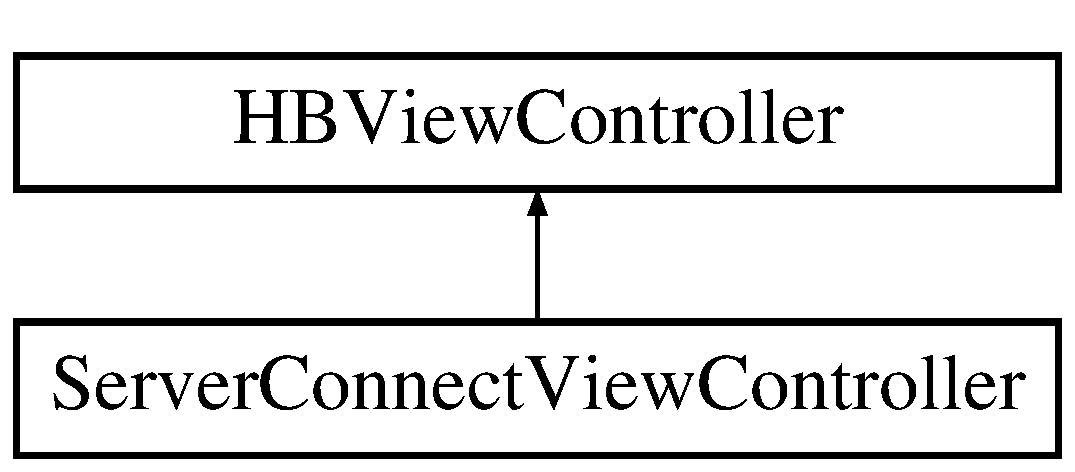
\includegraphics[height=2.000000cm]{class_server_connect_view_controller}
\end{center}
\end{figure}
\subsection*{Public Member Functions}
\begin{DoxyCompactItemize}
\item 
\hypertarget{class_server_connect_view_controller_adbe950a8af41236837cec1c151132f49}{H\-B\-View\-Mode {\bfseries did\-Finish\-View} ()}\label{class_server_connect_view_controller_adbe950a8af41236837cec1c151132f49}

\item 
\hypertarget{class_server_connect_view_controller_aab4ea172cba6914aa0d35d8ac5085e84}{void {\bfseries process} ()}\label{class_server_connect_view_controller_aab4ea172cba6914aa0d35d8ac5085e84}

\item 
\hypertarget{class_server_connect_view_controller_a608c67d2e278ae8ab5a95b5fef21dbc8}{void {\bfseries render} ()}\label{class_server_connect_view_controller_a608c67d2e278ae8ab5a95b5fef21dbc8}

\item 
\hypertarget{class_server_connect_view_controller_aedb4cdccaa547791f14c0db1634c82f6}{bool {\bfseries quit} ()}\label{class_server_connect_view_controller_aedb4cdccaa547791f14c0db1634c82f6}

\end{DoxyCompactItemize}


The documentation for this class was generated from the following files\-:\begin{DoxyCompactItemize}
\item 
Server\-Connect\-View\-Controller.\-h\item 
Server\-Connect\-View\-Controller.\-cpp\end{DoxyCompactItemize}

\hypertarget{classslidermenuitem}{\section{slidermenuitem Class Reference}
\label{classslidermenuitem}\index{slidermenuitem@{slidermenuitem}}
}
Inheritance diagram for slidermenuitem\-:\begin{figure}[H]
\begin{center}
\leavevmode
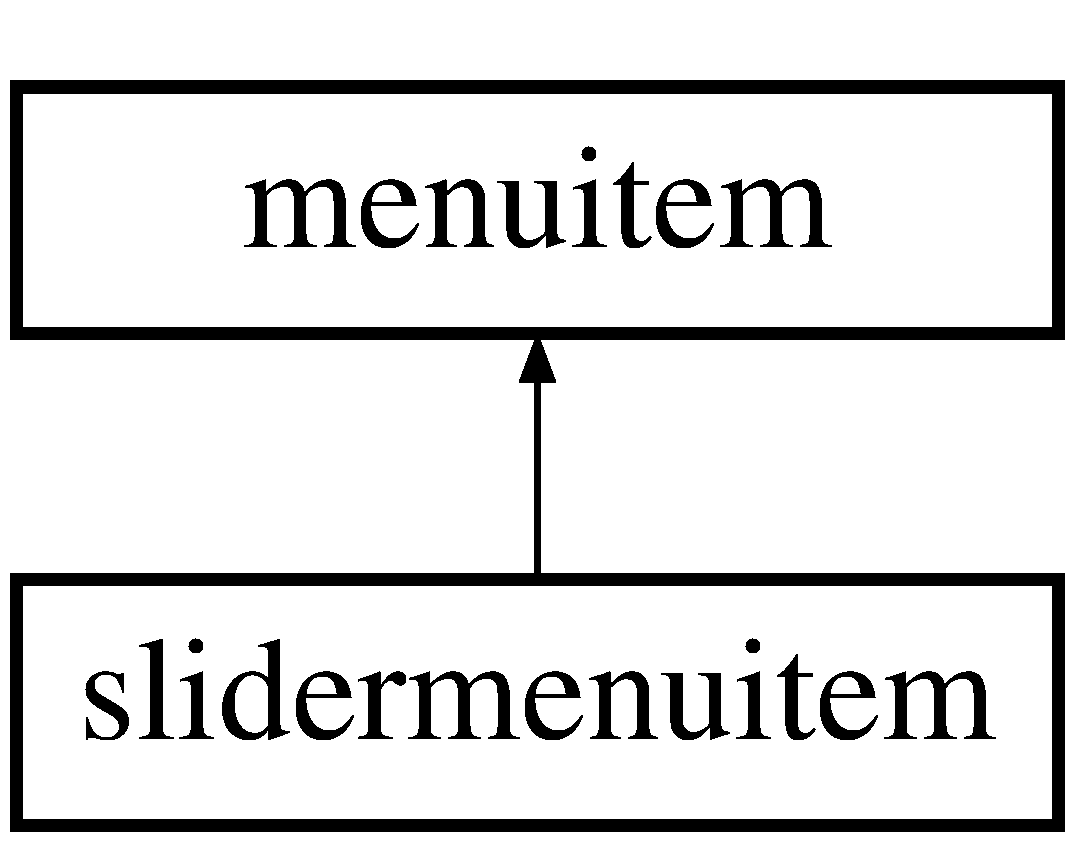
\includegraphics[height=2.000000cm]{classslidermenuitem}
\end{center}
\end{figure}
\subsection*{Public Member Functions}
\begin{DoxyCompactItemize}
\item 
\hypertarget{classslidermenuitem_a8d3ea3a2e8ffc77f6245f06403fb190b}{{\footnotesize template$<$class A $>$ }\\{\bfseries slidermenuitem} (char $\ast$name1, char $\ast$$\ast$states1, int len1, int curstate1, A act)}\label{classslidermenuitem_a8d3ea3a2e8ffc77f6245f06403fb190b}

\item 
\hypertarget{classslidermenuitem_acb7ab7077ab55851b6f9a0e45ebf5c56}{virtual void {\bfseries key\-\_\-input\-\_\-non\-\_\-active} (int key)}\label{classslidermenuitem_acb7ab7077ab55851b6f9a0e45ebf5c56}

\item 
\hypertarget{classslidermenuitem_ae07d0ff2b7111f833eeac63db401c2c7}{bool {\bfseries get\-\_\-state} ()}\label{classslidermenuitem_ae07d0ff2b7111f833eeac63db401c2c7}

\item 
\hypertarget{classslidermenuitem_a2e73d096c83aa1fb9f9a188a6c82c9a9}{virtual bool {\bfseries activate} ()}\label{classslidermenuitem_a2e73d096c83aa1fb9f9a188a6c82c9a9}

\item 
\hypertarget{classslidermenuitem_a62e992884ae1c6e4e44f1ebe5c84af5e}{virtual void {\bfseries draw} (bool, float, float, float, float, unsigned char)}\label{classslidermenuitem_a62e992884ae1c6e4e44f1ebe5c84af5e}

\item 
\hypertarget{classslidermenuitem_a5beb11932e734e3ee5285ff2d967d804}{virtual void {\bfseries on\-Deselect} ()}\label{classslidermenuitem_a5beb11932e734e3ee5285ff2d967d804}

\end{DoxyCompactItemize}


The documentation for this class was generated from the following files\-:\begin{DoxyCompactItemize}
\item 
menu.\-h\item 
menudraw.\-cpp\item 
menuitem.\-cpp\end{DoxyCompactItemize}

\hypertarget{class_socket}{\section{Socket Class Reference}
\label{class_socket}\index{Socket@{Socket}}
}
\subsection*{Public Member Functions}
\begin{DoxyCompactItemize}
\item 
\hyperlink{class_socket_acba9bcb13219372b3236ebd45edc29fb}{Socket} (int sock)
\item 
void \hyperlink{class_socket_a9409d7a46addea38d47d26ebe06bc93b}{listen\-\_\-for\-\_\-client} ()
\item 
class \hyperlink{class_socket_connection}{Socket\-Connection} $\ast$ \hyperlink{class_socket_a4637d93fff9965d3c93f20d091e15ce6}{receive\-Connection} ()
\item 
void \hyperlink{class_socket_ad9f8aabc5908fd1ba5383196e5dbb513}{close\-Connection} (\hyperlink{class_socket_connection}{Socket\-Connection} $\ast$sc)
\item 
class \hyperlink{class_socket_connection}{Socket\-Connection} $\ast$ \hyperlink{class_socket_a5f927294fc68ee16d297ced2dd5ed7e8}{connect} (sockaddr $\ast$addr, socklen\-\_\-t addrlen)
\item 
void \hyperlink{class_socket_a6c8618907b9b3395f18b9d15b4e4db03}{end\-\_\-connection} ()
\item 
void \hyperlink{class_socket_a924e09899ab24fb092b94ce03e17a6af}{recv\-\_\-all} ()
\end{DoxyCompactItemize}


\subsection{Constructor \& Destructor Documentation}
\hypertarget{class_socket_acba9bcb13219372b3236ebd45edc29fb}{\index{Socket@{Socket}!Socket@{Socket}}
\index{Socket@{Socket}!Socket@{Socket}}
\subsubsection[{Socket}]{\setlength{\rightskip}{0pt plus 5cm}{\bf Socket\-::\-Socket} (
\begin{DoxyParamCaption}
\item[{int}]{sock}
\end{DoxyParamCaption}
)}}\label{class_socket_acba9bcb13219372b3236ebd45edc29fb}
Creates a \hyperlink{class_socket}{Socket} class with the given socket descriptor, which must be of type S\-O\-C\-K\-\_\-\-D\-G\-R\-A\-M. 
\begin{DoxyParams}{Parameters}
{\em sock} & The socket descriptor, which must be of type S\-O\-C\-K\-\_\-\-D\-G\-R\-A\-M. \\
\hline
\end{DoxyParams}


\subsection{Member Function Documentation}
\hypertarget{class_socket_ad9f8aabc5908fd1ba5383196e5dbb513}{\index{Socket@{Socket}!close\-Connection@{close\-Connection}}
\index{close\-Connection@{close\-Connection}!Socket@{Socket}}
\subsubsection[{close\-Connection}]{\setlength{\rightskip}{0pt plus 5cm}void {\bf Socket\-::close\-Connection} (
\begin{DoxyParamCaption}
\item[{{\bf Socket\-Connection} $\ast$}]{sc}
\end{DoxyParamCaption}
)}}\label{class_socket_ad9f8aabc5908fd1ba5383196e5dbb513}
Closes the given \hyperlink{class_socket_connection}{Socket\-Connection}. 
\begin{DoxyParams}{Parameters}
{\em sc} & the \hyperlink{class_socket_connection}{Socket\-Connection} instance to be closed. \\
\hline
\end{DoxyParams}
\hypertarget{class_socket_a5f927294fc68ee16d297ced2dd5ed7e8}{\index{Socket@{Socket}!connect@{connect}}
\index{connect@{connect}!Socket@{Socket}}
\subsubsection[{connect}]{\setlength{\rightskip}{0pt plus 5cm}{\bf Socket\-Connection} $\ast$ {\bf Socket\-::connect} (
\begin{DoxyParamCaption}
\item[{sockaddr $\ast$}]{addr, }
\item[{socklen\-\_\-t}]{addrlen}
\end{DoxyParamCaption}
)}}\label{class_socket_a5f927294fc68ee16d297ced2dd5ed7e8}
Connects to the given address, and returns the resulting \hyperlink{class_socket_connection}{Socket\-Connection}. \begin{DoxyReturn}{Returns}
a \hyperlink{class_socket_connection}{Socket\-Connection} instance for the connection 
\end{DoxyReturn}
\hypertarget{class_socket_a6c8618907b9b3395f18b9d15b4e4db03}{\index{Socket@{Socket}!end\-\_\-connection@{end\-\_\-connection}}
\index{end\-\_\-connection@{end\-\_\-connection}!Socket@{Socket}}
\subsubsection[{end\-\_\-connection}]{\setlength{\rightskip}{0pt plus 5cm}void {\bf Socket\-::end\-\_\-connection} (
\begin{DoxyParamCaption}
{}
\end{DoxyParamCaption}
)}}\label{class_socket_a6c8618907b9b3395f18b9d15b4e4db03}
Closes everything \hypertarget{class_socket_a9409d7a46addea38d47d26ebe06bc93b}{\index{Socket@{Socket}!listen\-\_\-for\-\_\-client@{listen\-\_\-for\-\_\-client}}
\index{listen\-\_\-for\-\_\-client@{listen\-\_\-for\-\_\-client}!Socket@{Socket}}
\subsubsection[{listen\-\_\-for\-\_\-client}]{\setlength{\rightskip}{0pt plus 5cm}void {\bf Socket\-::listen\-\_\-for\-\_\-client} (
\begin{DoxyParamCaption}
{}
\end{DoxyParamCaption}
)}}\label{class_socket_a9409d7a46addea38d47d26ebe06bc93b}
Puts the \hyperlink{class_socket}{Socket} into listening mode. Should be used by a server who wants to listen for incoming connections with clients. \hypertarget{class_socket_a4637d93fff9965d3c93f20d091e15ce6}{\index{Socket@{Socket}!receive\-Connection@{receive\-Connection}}
\index{receive\-Connection@{receive\-Connection}!Socket@{Socket}}
\subsubsection[{receive\-Connection}]{\setlength{\rightskip}{0pt plus 5cm}{\bf Socket\-Connection} $\ast$ {\bf Socket\-::receive\-Connection} (
\begin{DoxyParamCaption}
{}
\end{DoxyParamCaption}
)}}\label{class_socket_a4637d93fff9965d3c93f20d091e15ce6}
Returns a new \hyperlink{class_socket_connection}{Socket\-Connection} that was received. New sockets can only be received if in listening mode. \begin{DoxyReturn}{Returns}
a new \hyperlink{class_socket_connection}{Socket\-Connection}, or N\-U\-L\-L if all received connections already been returned. 
\end{DoxyReturn}
\hypertarget{class_socket_a924e09899ab24fb092b94ce03e17a6af}{\index{Socket@{Socket}!recv\-\_\-all@{recv\-\_\-all}}
\index{recv\-\_\-all@{recv\-\_\-all}!Socket@{Socket}}
\subsubsection[{recv\-\_\-all}]{\setlength{\rightskip}{0pt plus 5cm}void {\bf Socket\-::recv\-\_\-all} (
\begin{DoxyParamCaption}
{}
\end{DoxyParamCaption}
)}}\label{class_socket_a924e09899ab24fb092b94ce03e17a6af}
Must be called periodically to process all incoming data to find new connections and pass this data to the Socket\-Connections. 

The documentation for this class was generated from the following files\-:\begin{DoxyCompactItemize}
\item 
socket.\-h\item 
socket.\-cpp\end{DoxyCompactItemize}

\hypertarget{class_socket_connection}{\section{Socket\-Connection Class Reference}
\label{class_socket_connection}\index{Socket\-Connection@{Socket\-Connection}}
}


The documentation for this class was generated from the following files\-:\begin{DoxyCompactItemize}
\item 
socket.\-h\item 
Socket\-Connection.\-cpp\end{DoxyCompactItemize}

\hypertarget{class_spawn}{\section{Spawn Class Reference}
\label{class_spawn}\index{Spawn@{Spawn}}
}
\subsection*{Public Member Functions}
\begin{DoxyCompactItemize}
\item 
\hypertarget{class_spawn_a195e12b95170a6c88d1e61b290a6678c}{{\bfseries Spawn} (float xmin, float xmax, float ymin, float ymax, float mass, float rad, \hyperlink{class_color}{Color} color, float hrat)}\label{class_spawn_a195e12b95170a6c88d1e61b290a6678c}

\end{DoxyCompactItemize}
\subsection*{Public Attributes}
\begin{DoxyCompactItemize}
\item 
\hypertarget{class_spawn_aeda64316c0a8ffca2da962cbd6e53de1}{float {\bfseries xmin}}\label{class_spawn_aeda64316c0a8ffca2da962cbd6e53de1}

\item 
\hypertarget{class_spawn_afd4c62cd67325dccfe7970bcb451409e}{float {\bfseries xmax}}\label{class_spawn_afd4c62cd67325dccfe7970bcb451409e}

\item 
\hypertarget{class_spawn_abcd0124e2b0d6b18f1240e1037b2d2ce}{float {\bfseries ymin}}\label{class_spawn_abcd0124e2b0d6b18f1240e1037b2d2ce}

\item 
\hypertarget{class_spawn_af3041b57a222968dcea6e0652d8e5c12}{float {\bfseries ymax}}\label{class_spawn_af3041b57a222968dcea6e0652d8e5c12}

\item 
\hypertarget{class_spawn_a228bf006bb6137fd632c238d9e876def}{float {\bfseries mass}}\label{class_spawn_a228bf006bb6137fd632c238d9e876def}

\item 
\hypertarget{class_spawn_a4521e63486a6cccbc110699c014ad95c}{float {\bfseries rad}}\label{class_spawn_a4521e63486a6cccbc110699c014ad95c}

\item 
\hypertarget{class_spawn_a1c3fca682e4a53b533a9c8b0b039b28a}{\hyperlink{class_color}{Color} {\bfseries color}}\label{class_spawn_a1c3fca682e4a53b533a9c8b0b039b28a}

\item 
\hypertarget{class_spawn_a02e45febfbb4ae0fc16f74395fc50018}{float {\bfseries hrat}}\label{class_spawn_a02e45febfbb4ae0fc16f74395fc50018}

\end{DoxyCompactItemize}


The documentation for this class was generated from the following file\-:\begin{DoxyCompactItemize}
\item 
hack.\-h\end{DoxyCompactItemize}

\hypertarget{class_splash_view_controller}{\section{Splash\-View\-Controller Class Reference}
\label{class_splash_view_controller}\index{Splash\-View\-Controller@{Splash\-View\-Controller}}
}
Inheritance diagram for Splash\-View\-Controller\-:\begin{figure}[H]
\begin{center}
\leavevmode
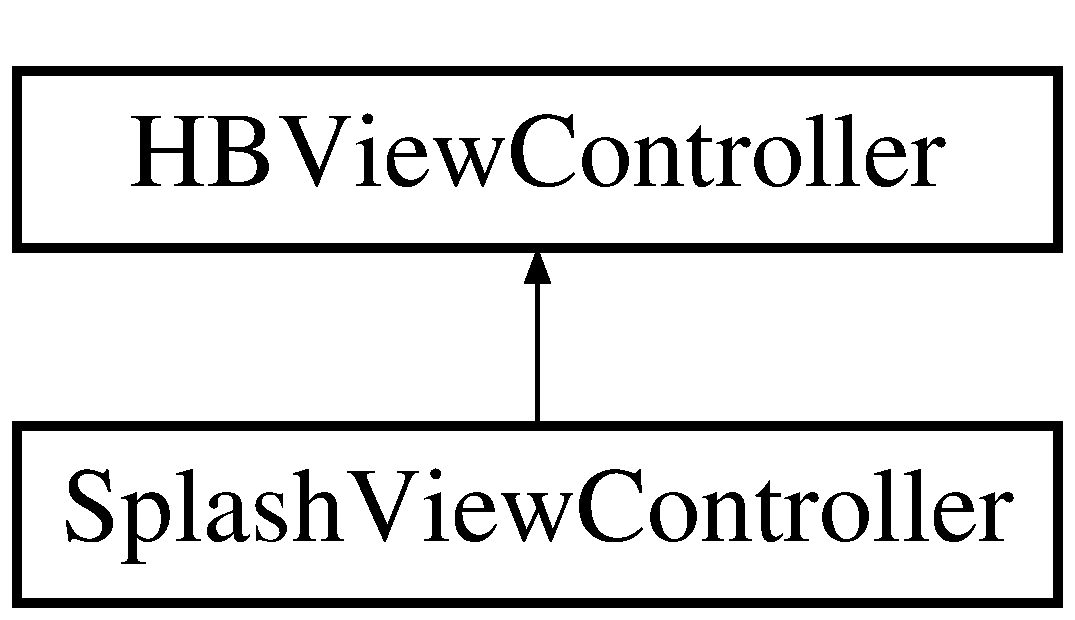
\includegraphics[height=2.000000cm]{class_splash_view_controller}
\end{center}
\end{figure}
\subsection*{Public Member Functions}
\begin{DoxyCompactItemize}
\item 
\hypertarget{class_splash_view_controller_aa537448267eb12a016f733dc029017ed}{H\-B\-View\-Mode {\bfseries did\-Finish\-View} ()}\label{class_splash_view_controller_aa537448267eb12a016f733dc029017ed}

\item 
\hypertarget{class_splash_view_controller_aca5b5fc1f60391ac72d1f2a31a7e13b5}{void {\bfseries process} ()}\label{class_splash_view_controller_aca5b5fc1f60391ac72d1f2a31a7e13b5}

\item 
\hypertarget{class_splash_view_controller_a2940ddcc3675b8e9f5b1902c8c176d3f}{void {\bfseries render} ()}\label{class_splash_view_controller_a2940ddcc3675b8e9f5b1902c8c176d3f}

\item 
\hypertarget{class_splash_view_controller_a9b0d10569eefc088ac627207f18db974}{bool {\bfseries quit} ()}\label{class_splash_view_controller_a9b0d10569eefc088ac627207f18db974}

\end{DoxyCompactItemize}


The documentation for this class was generated from the following files\-:\begin{DoxyCompactItemize}
\item 
Splash\-View\-Controller.\-h\item 
Splash\-View\-Controller.\-cpp\end{DoxyCompactItemize}

\hypertarget{class_string_tokenizer}{\section{String\-Tokenizer Class Reference}
\label{class_string_tokenizer}\index{String\-Tokenizer@{String\-Tokenizer}}
}
\subsection*{Public Member Functions}
\begin{DoxyCompactItemize}
\item 
\hypertarget{class_string_tokenizer_abe20997216d6c427b1c70ea92ffc58d1}{{\bfseries String\-Tokenizer} (std\-::string \&s, std\-::string delim=\char`\"{} $\backslash$t\char`\"{})}\label{class_string_tokenizer_abe20997216d6c427b1c70ea92ffc58d1}

\item 
\hypertarget{class_string_tokenizer_a3604c402ac9789b32f6446efadf348e0}{std\-::string {\bfseries next\-Token} ()}\label{class_string_tokenizer_a3604c402ac9789b32f6446efadf348e0}

\item 
\hypertarget{class_string_tokenizer_aae2b0616e31bf6342f3417677f2a2c83}{bool {\bfseries has\-More\-Tokens} () const }\label{class_string_tokenizer_aae2b0616e31bf6342f3417677f2a2c83}

\end{DoxyCompactItemize}


The documentation for this class was generated from the following file\-:\begin{DoxyCompactItemize}
\item 
H\-B\-Map.\-cpp\end{DoxyCompactItemize}

\hypertarget{classsubmenuitem}{\section{submenuitem Class Reference}
\label{classsubmenuitem}\index{submenuitem@{submenuitem}}
}
Inheritance diagram for submenuitem\-:\begin{figure}[H]
\begin{center}
\leavevmode
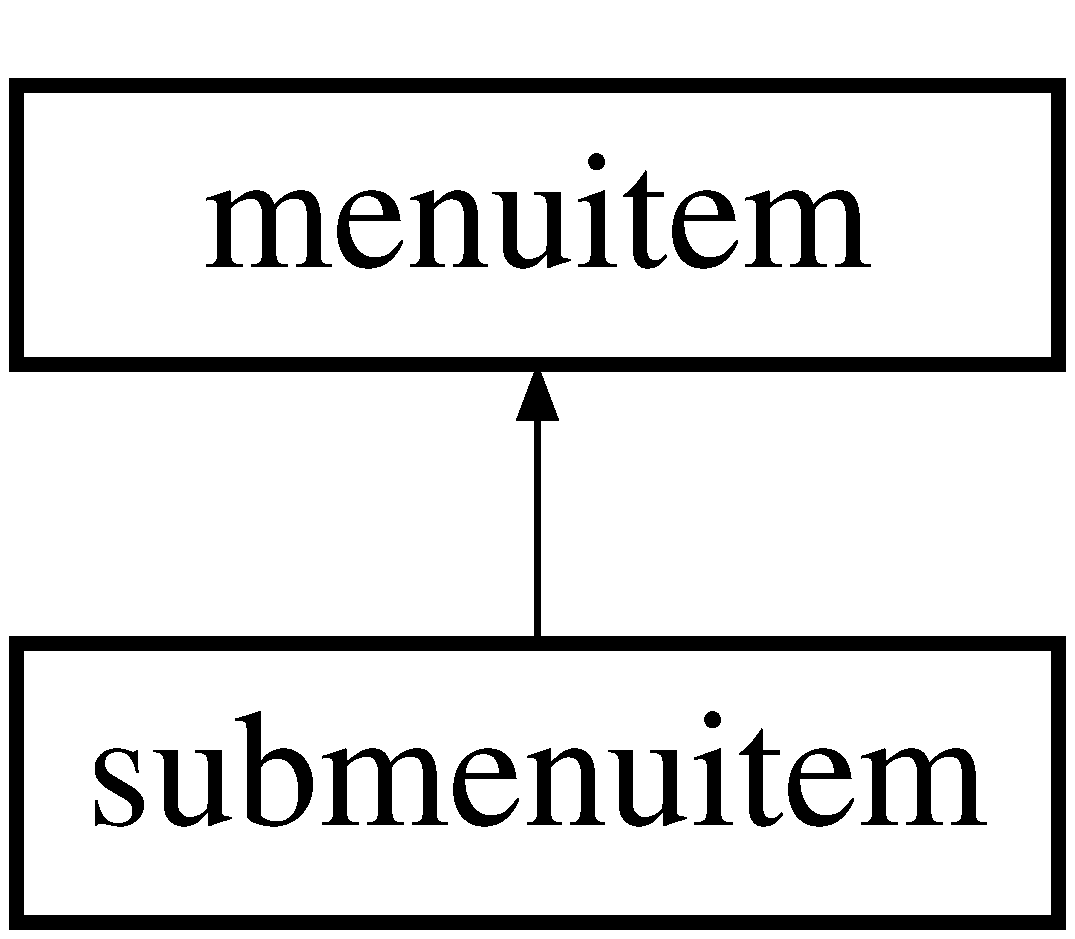
\includegraphics[height=2.000000cm]{classsubmenuitem}
\end{center}
\end{figure}
\subsection*{Public Member Functions}
\begin{DoxyCompactItemize}
\item 
\hypertarget{classsubmenuitem_a5b5cfc826ecfdd28bcadc5c4e0ab4e37}{{\bfseries submenuitem} (\hyperlink{classmenu}{menu} $\ast$m, char $\ast$name)}\label{classsubmenuitem_a5b5cfc826ecfdd28bcadc5c4e0ab4e37}

\item 
\hypertarget{classsubmenuitem_a5f2cc91e9d33890273b1e753243d083b}{virtual bool {\bfseries activate} ()}\label{classsubmenuitem_a5f2cc91e9d33890273b1e753243d083b}

\item 
\hypertarget{classsubmenuitem_ab270e28911151f45565ef5dd5843a1c3}{virtual bool {\bfseries key\-\_\-input} (int key)}\label{classsubmenuitem_ab270e28911151f45565ef5dd5843a1c3}

\item 
\hypertarget{classsubmenuitem_a8e9b02aa94b2047c2322f1d093ca7a86}{virtual void {\bfseries draw\-As\-Active} (unsigned char alpha)}\label{classsubmenuitem_a8e9b02aa94b2047c2322f1d093ca7a86}

\item 
\hypertarget{classsubmenuitem_ab8812b45b622f1d6ee2f7c0f35da08e9}{virtual bool {\bfseries should\-Menu\-Be\-Drawn} ()}\label{classsubmenuitem_ab8812b45b622f1d6ee2f7c0f35da08e9}

\item 
\hypertarget{classsubmenuitem_ae222458c62f3b2299b59db12cd71a2ec}{virtual void {\bfseries draw} (bool, float, float, float, float, unsigned char)}\label{classsubmenuitem_ae222458c62f3b2299b59db12cd71a2ec}

\end{DoxyCompactItemize}


The documentation for this class was generated from the following files\-:\begin{DoxyCompactItemize}
\item 
menu.\-h\item 
menudraw.\-cpp\item 
menuitem.\-cpp\end{DoxyCompactItemize}

\hypertarget{class_team}{\section{Team Class Reference}
\label{class_team}\index{Team@{Team}}
}
\subsection*{Public Member Functions}
\begin{DoxyCompactItemize}
\item 
\hyperlink{class_team_aada295895b747960576b69d8c87a54ba}{Team} ()
\item 
\hyperlink{class_team_af573698b380a45356b9688ef133ebb70}{Team} (unsigned a, unsigned b, unsigned c)
\item 
unsigned \hyperlink{class_team_a1f0a3f7266bae64a575fcabb957c52fd}{get\-Team\-Number} ()
\item 
unsigned \hyperlink{class_team_acf41227ed40aba5a75c3d3420fb77366}{get\-Min\-Players} ()
\item 
unsigned \hyperlink{class_team_accd137aa2bbf45c7251f447ebb02d9bc}{get\-Max\-Players} ()
\end{DoxyCompactItemize}


\subsection{Constructor \& Destructor Documentation}
\hypertarget{class_team_aada295895b747960576b69d8c87a54ba}{\index{Team@{Team}!Team@{Team}}
\index{Team@{Team}!Team@{Team}}
\subsubsection[{Team}]{\setlength{\rightskip}{0pt plus 5cm}{\bf Team\-::\-Team} (
\begin{DoxyParamCaption}
{}
\end{DoxyParamCaption}
)\hspace{0.3cm}{\ttfamily  \mbox{[}inline\mbox{]}}}}\label{class_team_aada295895b747960576b69d8c87a54ba}
Empty team constructor. Does nothing. \hypertarget{class_team_af573698b380a45356b9688ef133ebb70}{\index{Team@{Team}!Team@{Team}}
\index{Team@{Team}!Team@{Team}}
\subsubsection[{Team}]{\setlength{\rightskip}{0pt plus 5cm}{\bf Team\-::\-Team} (
\begin{DoxyParamCaption}
\item[{unsigned}]{a, }
\item[{unsigned}]{b, }
\item[{unsigned}]{c}
\end{DoxyParamCaption}
)\hspace{0.3cm}{\ttfamily  \mbox{[}inline\mbox{]}}}}\label{class_team_af573698b380a45356b9688ef133ebb70}
Constructs a team given the team number, minimum number of players, and maximum number of players.


\begin{DoxyParams}{Parameters}
{\em a} & the team number. \\
\hline
{\em b} & the minimum number of players. \\
\hline
{\em c} & the maximum number of players. \\
\hline
\end{DoxyParams}


\subsection{Member Function Documentation}
\hypertarget{class_team_accd137aa2bbf45c7251f447ebb02d9bc}{\index{Team@{Team}!get\-Max\-Players@{get\-Max\-Players}}
\index{get\-Max\-Players@{get\-Max\-Players}!Team@{Team}}
\subsubsection[{get\-Max\-Players}]{\setlength{\rightskip}{0pt plus 5cm}unsigned {\bf Team\-::get\-Max\-Players} (
\begin{DoxyParamCaption}
{}
\end{DoxyParamCaption}
)\hspace{0.3cm}{\ttfamily  \mbox{[}inline\mbox{]}}}}\label{class_team_accd137aa2bbf45c7251f447ebb02d9bc}
Gets the maximum number of players for this team.

\begin{DoxyReturn}{Returns}
the maximum number of players. 
\end{DoxyReturn}
\hypertarget{class_team_acf41227ed40aba5a75c3d3420fb77366}{\index{Team@{Team}!get\-Min\-Players@{get\-Min\-Players}}
\index{get\-Min\-Players@{get\-Min\-Players}!Team@{Team}}
\subsubsection[{get\-Min\-Players}]{\setlength{\rightskip}{0pt plus 5cm}unsigned {\bf Team\-::get\-Min\-Players} (
\begin{DoxyParamCaption}
{}
\end{DoxyParamCaption}
)\hspace{0.3cm}{\ttfamily  \mbox{[}inline\mbox{]}}}}\label{class_team_acf41227ed40aba5a75c3d3420fb77366}
Gets the minimum number of players for this team.

\begin{DoxyReturn}{Returns}
the minimum number of players. 
\end{DoxyReturn}
\hypertarget{class_team_a1f0a3f7266bae64a575fcabb957c52fd}{\index{Team@{Team}!get\-Team\-Number@{get\-Team\-Number}}
\index{get\-Team\-Number@{get\-Team\-Number}!Team@{Team}}
\subsubsection[{get\-Team\-Number}]{\setlength{\rightskip}{0pt plus 5cm}unsigned {\bf Team\-::get\-Team\-Number} (
\begin{DoxyParamCaption}
{}
\end{DoxyParamCaption}
)\hspace{0.3cm}{\ttfamily  \mbox{[}inline\mbox{]}}}}\label{class_team_a1f0a3f7266bae64a575fcabb957c52fd}
Gets the team number for this team.

\begin{DoxyReturn}{Returns}
the team number. 
\end{DoxyReturn}


The documentation for this class was generated from the following file\-:\begin{DoxyCompactItemize}
\item 
hack.\-h\end{DoxyCompactItemize}

\hypertarget{structtextquad}{\section{textquad Struct Reference}
\label{structtextquad}\index{textquad@{textquad}}
}
\subsection*{Public Member Functions}
\begin{DoxyCompactItemize}
\item 
\hypertarget{structtextquad_af57e4b44cc03271bfa6659492f2efc5f}{{\bfseries textquad} (float, float, float, float, float, float, float, float, float)}\label{structtextquad_af57e4b44cc03271bfa6659492f2efc5f}

\item 
\hypertarget{structtextquad_ae7d7ccac9ee4c8cab9bbfb75bdf84985}{void {\bfseries inc} (float s)}\label{structtextquad_ae7d7ccac9ee4c8cab9bbfb75bdf84985}

\end{DoxyCompactItemize}
\subsection*{Public Attributes}
\begin{DoxyCompactItemize}
\item 
\hypertarget{structtextquad_aa0712627d76a8d162e00645f56286de9}{float {\bfseries x1}}\label{structtextquad_aa0712627d76a8d162e00645f56286de9}

\item 
\hypertarget{structtextquad_aae86fe50b0bb27b5f82dcf26d34f395a}{float {\bfseries y1}}\label{structtextquad_aae86fe50b0bb27b5f82dcf26d34f395a}

\item 
\hypertarget{structtextquad_ac54c4d11a48300b0119298317d730fd4}{float {\bfseries z1}}\label{structtextquad_ac54c4d11a48300b0119298317d730fd4}

\item 
\hypertarget{structtextquad_ac3d5057748a416b2807666bbfb74b8cc}{float {\bfseries x2}}\label{structtextquad_ac3d5057748a416b2807666bbfb74b8cc}

\item 
\hypertarget{structtextquad_a4f9ed1b166d9d6833a857e10b582b582}{float {\bfseries y2}}\label{structtextquad_a4f9ed1b166d9d6833a857e10b582b582}

\item 
\hypertarget{structtextquad_a9dd8e2ac5ba0c3587384eca32b6d789f}{float {\bfseries z2}}\label{structtextquad_a9dd8e2ac5ba0c3587384eca32b6d789f}

\item 
\hypertarget{structtextquad_a8c8cb7b7a0b06e137481614692677b2c}{float {\bfseries dx}}\label{structtextquad_a8c8cb7b7a0b06e137481614692677b2c}

\item 
\hypertarget{structtextquad_a4b14cf2bee92820e3d54143010165279}{float {\bfseries dy}}\label{structtextquad_a4b14cf2bee92820e3d54143010165279}

\item 
\hypertarget{structtextquad_a0ba11d5b560b42898a3d39a885b46bac}{float {\bfseries dz}}\label{structtextquad_a0ba11d5b560b42898a3d39a885b46bac}

\end{DoxyCompactItemize}


The documentation for this struct was generated from the following files\-:\begin{DoxyCompactItemize}
\item 
font.\-h\item 
font.\-cpp\end{DoxyCompactItemize}

\hypertarget{class_texture}{\section{Texture Class Reference}
\label{class_texture}\index{Texture@{Texture}}
}
Inheritance diagram for Texture\-:\begin{figure}[H]
\begin{center}
\leavevmode
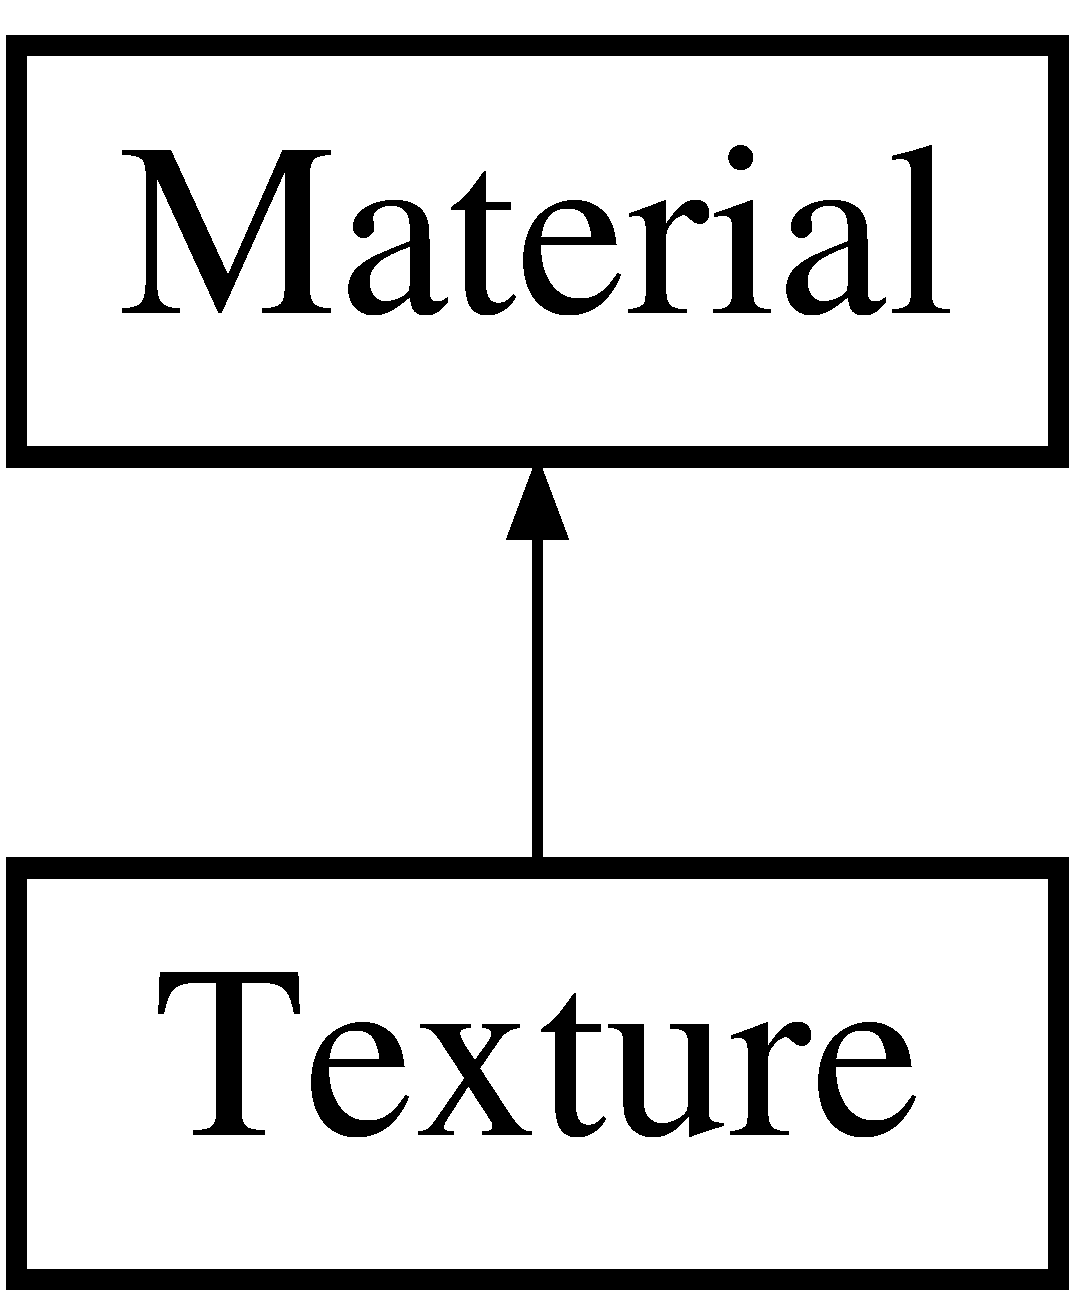
\includegraphics[height=2.000000cm]{class_texture}
\end{center}
\end{figure}


The documentation for this class was generated from the following file\-:\begin{DoxyCompactItemize}
\item 
Material.\-h\end{DoxyCompactItemize}

\hypertarget{classtogglemenuitem}{\section{togglemenuitem Class Reference}
\label{classtogglemenuitem}\index{togglemenuitem@{togglemenuitem}}
}
Inheritance diagram for togglemenuitem\-:\begin{figure}[H]
\begin{center}
\leavevmode
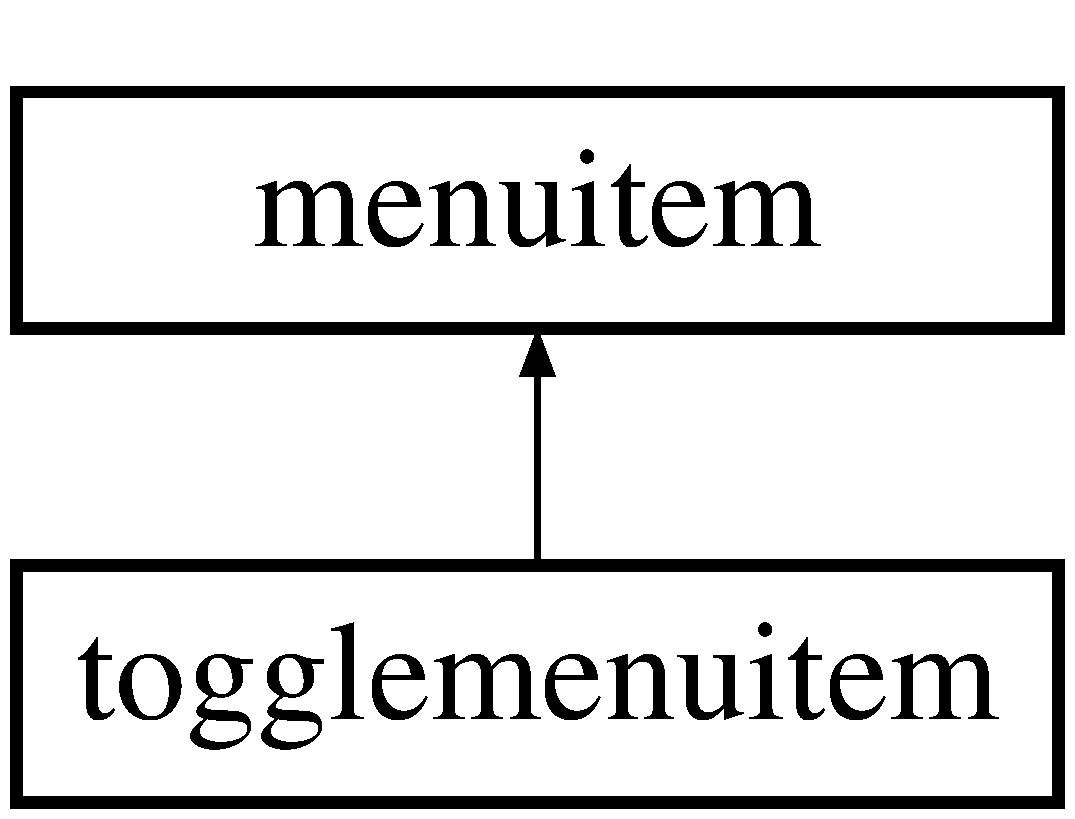
\includegraphics[height=2.000000cm]{classtogglemenuitem}
\end{center}
\end{figure}
\subsection*{Public Member Functions}
\begin{DoxyCompactItemize}
\item 
\hypertarget{classtogglemenuitem_a1e2cbb2a0b302aa58569aea49eef830c}{{\footnotesize template$<$class A $>$ }\\{\bfseries togglemenuitem} (char $\ast$name1, bool state1, A act)}\label{classtogglemenuitem_a1e2cbb2a0b302aa58569aea49eef830c}

\item 
\hypertarget{classtogglemenuitem_a43141175b333f427c408255708609f4d}{virtual bool {\bfseries activate} ()}\label{classtogglemenuitem_a43141175b333f427c408255708609f4d}

\item 
\hypertarget{classtogglemenuitem_a56ba78d7ca02ff2ef4a2e0b6e8782ebc}{bool {\bfseries get\-\_\-state} ()}\label{classtogglemenuitem_a56ba78d7ca02ff2ef4a2e0b6e8782ebc}

\item 
\hypertarget{classtogglemenuitem_a9245f46eca199c9d5b2c8bc494c1b737}{virtual void {\bfseries draw} (bool selected, float x1, float y1, float width, float height, unsigned char alpha)}\label{classtogglemenuitem_a9245f46eca199c9d5b2c8bc494c1b737}

\end{DoxyCompactItemize}


The documentation for this class was generated from the following files\-:\begin{DoxyCompactItemize}
\item 
menu.\-h\item 
menudraw.\-cpp\item 
menuitem.\-cpp\end{DoxyCompactItemize}

\hypertarget{class_unholy_game_view_controller}{\section{Unholy\-Game\-View\-Controller Class Reference}
\label{class_unholy_game_view_controller}\index{Unholy\-Game\-View\-Controller@{Unholy\-Game\-View\-Controller}}
}
Inheritance diagram for Unholy\-Game\-View\-Controller\-:\begin{figure}[H]
\begin{center}
\leavevmode
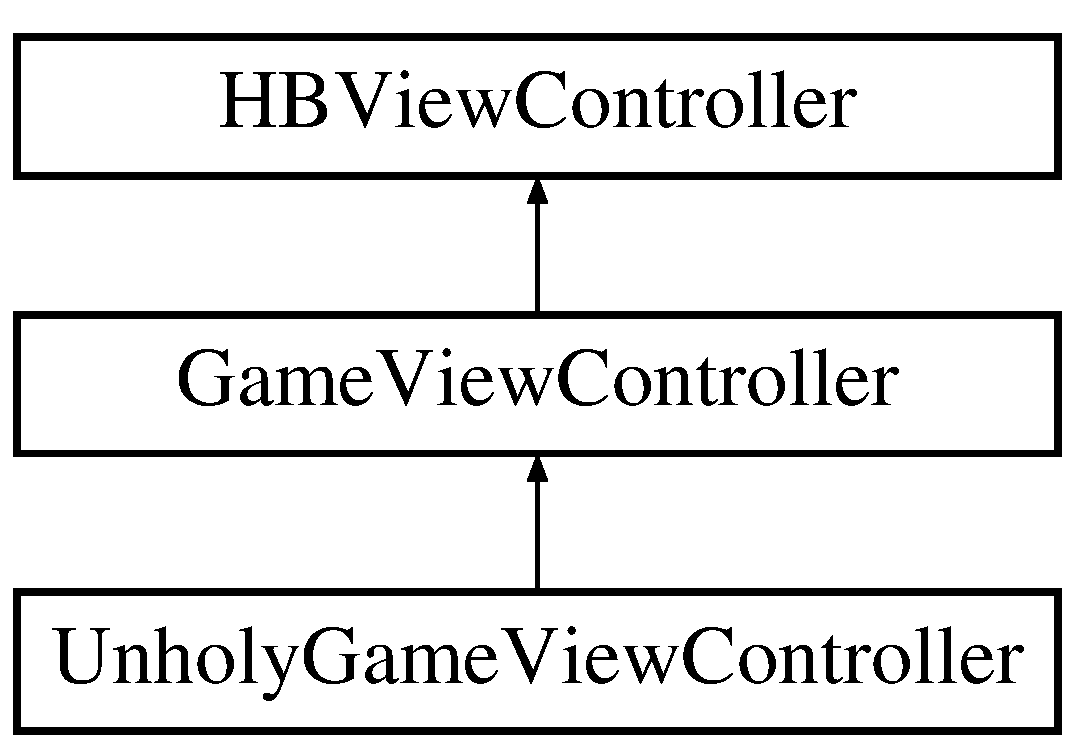
\includegraphics[height=3.000000cm]{class_unholy_game_view_controller}
\end{center}
\end{figure}
\subsection*{Public Member Functions}
\begin{DoxyCompactItemize}
\item 
\hypertarget{class_unholy_game_view_controller_a52f2297f438597e575049f066683f78a}{void {\bfseries process} ()}\label{class_unholy_game_view_controller_a52f2297f438597e575049f066683f78a}

\item 
\hypertarget{class_unholy_game_view_controller_a15d9253674a9c6a10f9196611bfe1b07}{void {\bfseries render} ()}\label{class_unholy_game_view_controller_a15d9253674a9c6a10f9196611bfe1b07}

\end{DoxyCompactItemize}


The documentation for this class was generated from the following files\-:\begin{DoxyCompactItemize}
\item 
Unholy\-Game\-View\-Controller.\-h\item 
Unholy\-Game\-View\-Controller.\-cpp\end{DoxyCompactItemize}

\hypertarget{class_vector2_d}{\section{Vector2\-D Class Reference}
\label{class_vector2_d}\index{Vector2\-D@{Vector2\-D}}
}
\subsection*{Public Member Functions}
\begin{DoxyCompactItemize}
\item 
\hypertarget{class_vector2_d_a25f848a3d2e7918eb8b1b7f3bcbe8b80}{{\bfseries Vector2\-D} (float a=0, float b=0)}\label{class_vector2_d_a25f848a3d2e7918eb8b1b7f3bcbe8b80}

\item 
\hypertarget{class_vector2_d_a8326913d685062bfb06abc8f041d0eb4}{\hyperlink{class_vector2_d}{Vector2\-D} {\bfseries operator+} (const \hyperlink{class_vector2_d}{Vector2\-D} \&) const }\label{class_vector2_d_a8326913d685062bfb06abc8f041d0eb4}

\item 
\hypertarget{class_vector2_d_a8c60be1594b61abfe6a4c155be8f8d5d}{\hyperlink{class_vector2_d}{Vector2\-D} {\bfseries operator-\/} (const \hyperlink{class_vector2_d}{Vector2\-D} \&) const }\label{class_vector2_d_a8c60be1594b61abfe6a4c155be8f8d5d}

\item 
\hypertarget{class_vector2_d_a6a92d36f310fbaefb2b3455f4dcd8820}{\hyperlink{class_vector2_d}{Vector2\-D} {\bfseries operator-\/} () const }\label{class_vector2_d_a6a92d36f310fbaefb2b3455f4dcd8820}

\item 
\hypertarget{class_vector2_d_afa7564ddcd8e27d95f1b9bed7772cdde}{\hyperlink{class_vector2_d}{Vector2\-D} \& {\bfseries operator+=} (const \hyperlink{class_vector2_d}{Vector2\-D} \&)}\label{class_vector2_d_afa7564ddcd8e27d95f1b9bed7772cdde}

\item 
\hypertarget{class_vector2_d_aba680626aa578eeb6e152840ffada6f5}{\hyperlink{class_vector2_d}{Vector2\-D} \& {\bfseries operator-\/=} (const \hyperlink{class_vector2_d}{Vector2\-D} \&)}\label{class_vector2_d_aba680626aa578eeb6e152840ffada6f5}

\item 
\hypertarget{class_vector2_d_a868c5c3253ff3c90a2836a378ef3eb18}{\hyperlink{class_vector2_d}{Vector2\-D} \& {\bfseries operator$\ast$=} (const float)}\label{class_vector2_d_a868c5c3253ff3c90a2836a378ef3eb18}

\item 
\hypertarget{class_vector2_d_aaaa3859e5b2387804433ab3c6f0d4195}{bool {\bfseries operator==} (const \hyperlink{class_vector2_d}{Vector2\-D} \&) const }\label{class_vector2_d_aaaa3859e5b2387804433ab3c6f0d4195}

\item 
\hypertarget{class_vector2_d_a8ef79708aada9d64f6e35f2f07d80dc1}{float {\bfseries operator$\ast$} (const \hyperlink{class_vector2_d}{Vector2\-D} \&) const }\label{class_vector2_d_a8ef79708aada9d64f6e35f2f07d80dc1}

\item 
\hypertarget{class_vector2_d_ac6b31ce90fa1e8bad9b26ffe409c26ed}{\hyperlink{class_vector2_d}{Vector2\-D} {\bfseries operator$\ast$} (const float) const }\label{class_vector2_d_ac6b31ce90fa1e8bad9b26ffe409c26ed}

\item 
\hypertarget{class_vector2_d_a71c67fe20a71ee7eeb96aa93c528d092}{\hyperlink{class_vector2_d}{Vector2\-D} {\bfseries get\-Normal\-Vector} () const }\label{class_vector2_d_a71c67fe20a71ee7eeb96aa93c528d092}

\end{DoxyCompactItemize}
\subsection*{Public Attributes}
\begin{DoxyCompactItemize}
\item 
\hypertarget{class_vector2_d_aeb4253ba6555251d010ea4450619029e}{float {\bfseries x}}\label{class_vector2_d_aeb4253ba6555251d010ea4450619029e}

\item 
\hypertarget{class_vector2_d_a85215519d3f71d0e6be7d636346f3b7d}{float {\bfseries y}}\label{class_vector2_d_a85215519d3f71d0e6be7d636346f3b7d}

\end{DoxyCompactItemize}


The documentation for this class was generated from the following files\-:\begin{DoxyCompactItemize}
\item 
hack.\-h\item 
vec.\-cpp\end{DoxyCompactItemize}

\hypertarget{class_vector3_d}{\section{Vector3\-D Class Reference}
\label{class_vector3_d}\index{Vector3\-D@{Vector3\-D}}
}
\subsection*{Public Member Functions}
\begin{DoxyCompactItemize}
\item 
\hypertarget{class_vector3_d_a30aeeb737a0982efdba3b0942aaf1c9e}{{\bfseries Vector3\-D} (float a=0, float b=0, float c=0)}\label{class_vector3_d_a30aeeb737a0982efdba3b0942aaf1c9e}

\item 
\hypertarget{class_vector3_d_ad9cb2ecfe33b2ad7fd23f9d24d606ab5}{{\bfseries Vector3\-D} (\hyperlink{class_vector2_d}{Vector2\-D} \&v)}\label{class_vector3_d_ad9cb2ecfe33b2ad7fd23f9d24d606ab5}

\item 
\hypertarget{class_vector3_d_a5c0a69fd6181b90fe3dffe6507386fe9}{\hyperlink{class_vector3_d}{Vector3\-D} {\bfseries operator+} (const \hyperlink{class_vector3_d}{Vector3\-D} \&) const }\label{class_vector3_d_a5c0a69fd6181b90fe3dffe6507386fe9}

\item 
\hypertarget{class_vector3_d_add4e475057a8fa5e1cd982fedad79827}{\hyperlink{class_vector3_d}{Vector3\-D} {\bfseries operator-\/} (const \hyperlink{class_vector3_d}{Vector3\-D} \&) const }\label{class_vector3_d_add4e475057a8fa5e1cd982fedad79827}

\item 
\hypertarget{class_vector3_d_a03f189f8d45eda497772364d19d30c7d}{\hyperlink{class_vector3_d}{Vector3\-D} {\bfseries operator-\/} () const }\label{class_vector3_d_a03f189f8d45eda497772364d19d30c7d}

\item 
\hypertarget{class_vector3_d_a878a97733a49fe99b7836475d5b1cf7d}{\hyperlink{class_vector3_d}{Vector3\-D} \& {\bfseries operator+=} (const \hyperlink{class_vector3_d}{Vector3\-D} \&)}\label{class_vector3_d_a878a97733a49fe99b7836475d5b1cf7d}

\item 
\hypertarget{class_vector3_d_a8facd6e805d6618eb2e2d5c04ec7b903}{\hyperlink{class_vector3_d}{Vector3\-D} \& {\bfseries operator-\/=} (const \hyperlink{class_vector3_d}{Vector3\-D} \&)}\label{class_vector3_d_a8facd6e805d6618eb2e2d5c04ec7b903}

\item 
\hypertarget{class_vector3_d_acb8297df60cafc9b31d32f39db0e2f8b}{\hyperlink{class_vector3_d}{Vector3\-D} \& {\bfseries operator$\ast$=} (const float)}\label{class_vector3_d_acb8297df60cafc9b31d32f39db0e2f8b}

\item 
\hypertarget{class_vector3_d_a5199dd8f778deff72cc929e5cf1ed471}{bool {\bfseries operator==} (const \hyperlink{class_vector3_d}{Vector3\-D} \&) const }\label{class_vector3_d_a5199dd8f778deff72cc929e5cf1ed471}

\item 
\hypertarget{class_vector3_d_a18db3e0452fd43081187dc4322c65c80}{float {\bfseries operator$\ast$} (const \hyperlink{class_vector3_d}{Vector3\-D}) const }\label{class_vector3_d_a18db3e0452fd43081187dc4322c65c80}

\item 
\hypertarget{class_vector3_d_a373000c84c9aa81d848e3f249bd0bd10}{\hyperlink{class_vector3_d}{Vector3\-D} {\bfseries operator$\ast$} (const float) const }\label{class_vector3_d_a373000c84c9aa81d848e3f249bd0bd10}

\end{DoxyCompactItemize}
\subsection*{Public Attributes}
\begin{DoxyCompactItemize}
\item 
\hypertarget{class_vector3_d_aca5d15bdb846448e3cb73b072783f329}{float {\bfseries x}}\label{class_vector3_d_aca5d15bdb846448e3cb73b072783f329}

\item 
\hypertarget{class_vector3_d_a9b6d194fcf526d7d4f9e902421285e94}{float {\bfseries y}}\label{class_vector3_d_a9b6d194fcf526d7d4f9e902421285e94}

\item 
\hypertarget{class_vector3_d_af9728f1eba23b9ee091755346214f391}{float {\bfseries z}}\label{class_vector3_d_af9728f1eba23b9ee091755346214f391}

\item 
\hypertarget{class_vector3_d_a7d7b3447b843474b2e6944388294f018}{float {\bfseries w}}\label{class_vector3_d_a7d7b3447b843474b2e6944388294f018}

\end{DoxyCompactItemize}


The documentation for this class was generated from the following files\-:\begin{DoxyCompactItemize}
\item 
hack.\-h\item 
vec.\-cpp\end{DoxyCompactItemize}

\hypertarget{structvoidtype}{\section{voidtype Struct Reference}
\label{structvoidtype}\index{voidtype@{voidtype}}
}


The documentation for this struct was generated from the following file\-:\begin{DoxyCompactItemize}
\item 
menu.\-h\end{DoxyCompactItemize}

\hypertarget{class_world}{\section{World Class Reference}
\label{class_world}\index{World@{World}}
}
\subsection*{Public Member Functions}
\begin{DoxyCompactItemize}
\item 
\hyperlink{class_world_a927865dd19c6a03b0d3b481ae03775c3}{World} (std\-::string map\-Name=\char`\"{}custom.\-hbm\char`\"{})
\item 
\hypertarget{class_world_af852886a613927fb0e1ca4b33a14f303}{int {\bfseries spawn} (int spawnl, int player, int flag)}\label{class_world_af852886a613927fb0e1ca4b33a14f303}

\item 
const float \hyperlink{class_world_a1780684e06f60af5a22bd232916860d8}{get\-Min\-X} () const 
\item 
const float \hyperlink{class_world_a1e35597fd94c241b9df7a87e9b6a523d}{get\-Max\-X} () const 
\item 
const float \hyperlink{class_world_a8ec2876af6bcbe4603c786eb67b040fd}{get\-Min\-Y} () const 
\item 
const float \hyperlink{class_world_a402581ee124acda99859c7e67edff1de}{get\-Max\-Y} () const 
\item 
\hypertarget{class_world_a587f1be5d3b3237a5c00714ec17e39a9}{void {\bfseries do\-Simulation} (float dt, std\-::vector$<$ std\-::pair$<$ char, \hyperlink{class_vector2_d}{Vector2\-D} $>$ $>$ \&sounds)}\label{class_world_a587f1be5d3b3237a5c00714ec17e39a9}

\item 
\hypertarget{class_world_ada6d1ec2f526a8529a709f5ce6fa2a0a}{void {\bfseries send\-Objects} (\hyperlink{class_socket_connection}{Socket\-Connection} $\ast$sc, int obj)}\label{class_world_ada6d1ec2f526a8529a709f5ce6fa2a0a}

\item 
\hypertarget{class_world_a2235107a1f2470dc270c2bfa3cf0ac51}{void {\bfseries receive\-Objects} (\hyperlink{class_read_packet}{Read\-Packet} $\ast$rp, int \&obj)}\label{class_world_a2235107a1f2470dc270c2bfa3cf0ac51}

\end{DoxyCompactItemize}
\subsection*{Public Attributes}
\begin{DoxyCompactItemize}
\item 
\hypertarget{class_world_a4ed3ad3160ad21a961c010dc2d10c4cf}{std\-::map$<$ int, std\-::vector\\*
$<$ \hyperlink{class_spawn}{Spawn} $>$ $>$ {\bfseries spawns}}\label{class_world_a4ed3ad3160ad21a961c010dc2d10c4cf}

\item 
\hypertarget{class_world_aa7f46be731fc0dd306f7f7d12c2407c2}{std\-::map$<$ int, \hyperlink{class_object}{Object} $>$ {\bfseries objects}}\label{class_world_aa7f46be731fc0dd306f7f7d12c2407c2}

\item 
\hypertarget{class_world_ab97ac12fd82256884dbbbd09a18d01c4}{std\-::vector$<$ \hyperlink{class_light}{Light} $>$ {\bfseries lights}}\label{class_world_ab97ac12fd82256884dbbbd09a18d01c4}

\item 
\hypertarget{class_world_acaee24cc3256bf5bc39147a326520655}{std\-::vector$<$ \hyperlink{class_obstacle}{Obstacle} $>$ {\bfseries obstacles}}\label{class_world_acaee24cc3256bf5bc39147a326520655}

\end{DoxyCompactItemize}


\subsection{Constructor \& Destructor Documentation}
\hypertarget{class_world_a927865dd19c6a03b0d3b481ae03775c3}{\index{World@{World}!World@{World}}
\index{World@{World}!World@{World}}
\subsubsection[{World}]{\setlength{\rightskip}{0pt plus 5cm}{\bf World\-::\-World} (
\begin{DoxyParamCaption}
\item[{std\-::string}]{map\-Name = {\ttfamily \char`\"{}custom.hbm\char`\"{}}}
\end{DoxyParamCaption}
)}}\label{class_world_a927865dd19c6a03b0d3b481ae03775c3}
Default constructor for \hyperlink{class_world}{World} given a map name from which to load the world.


\begin{DoxyParams}{Parameters}
{\em map\-Name} & the map file name. Defaults to \char`\"{}custom.\-hbm\char`\"{}. \\
\hline
\end{DoxyParams}


\subsection{Member Function Documentation}
\hypertarget{class_world_a1e35597fd94c241b9df7a87e9b6a523d}{\index{World@{World}!get\-Max\-X@{get\-Max\-X}}
\index{get\-Max\-X@{get\-Max\-X}!World@{World}}
\subsubsection[{get\-Max\-X}]{\setlength{\rightskip}{0pt plus 5cm}const float {\bf World\-::get\-Max\-X} (
\begin{DoxyParamCaption}
{}
\end{DoxyParamCaption}
) const\hspace{0.3cm}{\ttfamily  \mbox{[}inline\mbox{]}}}}\label{class_world_a1e35597fd94c241b9df7a87e9b6a523d}
Returns the maximum x coordinate of the world.

\begin{DoxyReturn}{Returns}
the maximum x coordinate. 
\end{DoxyReturn}
\hypertarget{class_world_a402581ee124acda99859c7e67edff1de}{\index{World@{World}!get\-Max\-Y@{get\-Max\-Y}}
\index{get\-Max\-Y@{get\-Max\-Y}!World@{World}}
\subsubsection[{get\-Max\-Y}]{\setlength{\rightskip}{0pt plus 5cm}const float {\bf World\-::get\-Max\-Y} (
\begin{DoxyParamCaption}
{}
\end{DoxyParamCaption}
) const\hspace{0.3cm}{\ttfamily  \mbox{[}inline\mbox{]}}}}\label{class_world_a402581ee124acda99859c7e67edff1de}
Returns the maximum y coordinate of the world.

\begin{DoxyReturn}{Returns}
the maximum y coordinate. 
\end{DoxyReturn}
\hypertarget{class_world_a1780684e06f60af5a22bd232916860d8}{\index{World@{World}!get\-Min\-X@{get\-Min\-X}}
\index{get\-Min\-X@{get\-Min\-X}!World@{World}}
\subsubsection[{get\-Min\-X}]{\setlength{\rightskip}{0pt plus 5cm}const float {\bf World\-::get\-Min\-X} (
\begin{DoxyParamCaption}
{}
\end{DoxyParamCaption}
) const\hspace{0.3cm}{\ttfamily  \mbox{[}inline\mbox{]}}}}\label{class_world_a1780684e06f60af5a22bd232916860d8}
Returns the minimum x coordinate of the world.

\begin{DoxyReturn}{Returns}
the minimum x coordinate. 
\end{DoxyReturn}
\hypertarget{class_world_a8ec2876af6bcbe4603c786eb67b040fd}{\index{World@{World}!get\-Min\-Y@{get\-Min\-Y}}
\index{get\-Min\-Y@{get\-Min\-Y}!World@{World}}
\subsubsection[{get\-Min\-Y}]{\setlength{\rightskip}{0pt plus 5cm}const float {\bf World\-::get\-Min\-Y} (
\begin{DoxyParamCaption}
{}
\end{DoxyParamCaption}
) const\hspace{0.3cm}{\ttfamily  \mbox{[}inline\mbox{]}}}}\label{class_world_a8ec2876af6bcbe4603c786eb67b040fd}
Returns the minimum y coordinate of the world.

\begin{DoxyReturn}{Returns}
the minimum y coordinate. 
\end{DoxyReturn}


The documentation for this class was generated from the following files\-:\begin{DoxyCompactItemize}
\item 
world.\-h\item 
simulate.\-cpp\item 
world.\-cpp\end{DoxyCompactItemize}

\hypertarget{classwrappedfuncobj}{\section{wrappedfuncobj$<$ R, I $>$ Class Template Reference}
\label{classwrappedfuncobj}\index{wrappedfuncobj$<$ R, I $>$@{wrappedfuncobj$<$ R, I $>$}}
}
\subsection*{Public Member Functions}
\begin{DoxyCompactItemize}
\item 
\hypertarget{classwrappedfuncobj_a68469ec527666fb4d485dd88f9217267}{{\bfseries wrappedfuncobj} (const \hyperlink{classwrappedfuncobj}{wrappedfuncobj}$<$ R, I $>$ \&to\-Copy)}\label{classwrappedfuncobj_a68469ec527666fb4d485dd88f9217267}

\item 
\hypertarget{classwrappedfuncobj_ac338e00331090276dca1d79615e42e33}{{\footnotesize template$<$class A $>$ }\\{\bfseries wrappedfuncobj} (A internal)}\label{classwrappedfuncobj_ac338e00331090276dca1d79615e42e33}

\item 
\hypertarget{classwrappedfuncobj_ac15f4caae45532d2ed29b48de235cf56}{\hyperlink{classwrappedfuncobj}{wrappedfuncobj} \& {\bfseries operator=} (const \hyperlink{classwrappedfuncobj}{wrappedfuncobj} \&to\-Copy)}\label{classwrappedfuncobj_ac15f4caae45532d2ed29b48de235cf56}

\item 
\hypertarget{classwrappedfuncobj_a26203fd381708305368d50300b95b77b}{R {\bfseries operator()} (I i)}\label{classwrappedfuncobj_a26203fd381708305368d50300b95b77b}

\end{DoxyCompactItemize}
\subsubsection*{template$<$class R, class I$>$ class wrappedfuncobj$<$ R, I $>$}



The documentation for this class was generated from the following file\-:\begin{DoxyCompactItemize}
\item 
menu.\-h\end{DoxyCompactItemize}

\hypertarget{class_write_packet}{\section{Write\-Packet Class Reference}
\label{class_write_packet}\index{Write\-Packet@{Write\-Packet}}
}
\subsection*{Public Member Functions}
\begin{DoxyCompactItemize}
\item 
\hypertarget{class_write_packet_aeac19c767326156d7c25747e396042b5}{{\bfseries Write\-Packet} (char message\-\_\-type, int max\-\_\-size=1)}\label{class_write_packet_aeac19c767326156d7c25747e396042b5}

\item 
\hypertarget{class_write_packet_a915f8d2b8715edbfe375c95ab2cdc891}{void {\bfseries write\-\_\-char} (char c)}\label{class_write_packet_a915f8d2b8715edbfe375c95ab2cdc891}

\item 
\hypertarget{class_write_packet_ab684b0f55e8dede898e13ce46c1d49db}{void {\bfseries write\-\_\-int} (int i)}\label{class_write_packet_ab684b0f55e8dede898e13ce46c1d49db}

\item 
\hypertarget{class_write_packet_a59548dc2e66dd2cd1a6cdcb5678d1308}{void {\bfseries write\-\_\-short} (short s)}\label{class_write_packet_a59548dc2e66dd2cd1a6cdcb5678d1308}

\item 
\hypertarget{class_write_packet_a0679dc68fb049c8bb0680bcdd3fbcf7d}{void {\bfseries write\-\_\-float} (float f)}\label{class_write_packet_a0679dc68fb049c8bb0680bcdd3fbcf7d}

\item 
\hypertarget{class_write_packet_a7c09c4008d359e2d7f56499a4c5ee5f6}{void {\bfseries write\-\_\-string} (std\-::string s)}\label{class_write_packet_a7c09c4008d359e2d7f56499a4c5ee5f6}

\end{DoxyCompactItemize}
\subsection*{Public Attributes}
\begin{DoxyCompactItemize}
\item 
\hypertarget{class_write_packet_a4e09d7a56020f0498198559b321b432a}{int {\bfseries max\-\_\-size}}\label{class_write_packet_a4e09d7a56020f0498198559b321b432a}

\item 
\hypertarget{class_write_packet_a5e064b121ff8ae689e3895abc6b6a66e}{int {\bfseries size}}\label{class_write_packet_a5e064b121ff8ae689e3895abc6b6a66e}

\item 
\hypertarget{class_write_packet_ac5ab6aac77c2c1e543c4abb10ab33e2a}{char $\ast$ {\bfseries buf}}\label{class_write_packet_ac5ab6aac77c2c1e543c4abb10ab33e2a}

\item 
\hypertarget{class_write_packet_ad916bc47670dd08982ab44b384396495}{char {\bfseries message\-\_\-type}}\label{class_write_packet_ad916bc47670dd08982ab44b384396495}

\end{DoxyCompactItemize}


The documentation for this class was generated from the following files\-:\begin{DoxyCompactItemize}
\item 
packet.\-h\item 
packet.\-cpp\end{DoxyCompactItemize}

\printindex
\end{document}
